\setchapterpreamble[u]{\margintoc}
\chapter{Garbage Collection}
\labch{garbage-collection}

\renewcommand{\lang}{\textsf{BFAE}\xspace}

Consider the following \lang expression:

$
\begin{array}{@{}l@{}}
  \ebind{\code{f}}{\efun{\code{x}}{( \\
  \ \ \ \ \eseq{\eref{\code{x}}}{ \\
  \ \ \ \ \code{x}} \\
  )}}{\\
  \eseq{\eapp{\code{f}}{0}}{ \\
  \eseq{\eapp{\code{f}}{1}}{ \\
  \cdots \\
  \eapp{\code{f}}{999}
  }}}
\end{array}
$

The function \code{f} creates a new box but does not use the box at all. Each
time the function is called, it newly creates one more box. The above expression
calls \code{f} 1,000 times, so there are 1,000 boxes in the store at the end of
the execution.

Under the operational semantics we have defined, programs like the above
expression are not problematic. The size of a store is unlimited, so each
program can create boxes as many as it wants.

However, the operational semantics does not fully reflect the execution of
programs on real machines; our semantics is merely a mathematical one. The
memory of every machine has a physical limit. There is a maximum number of boxes
that can be created on a single machine. Programs cannot create boxes forever.

How can we handle a situation that programs need to create boxes exceeding the
physical limit of the machine on which they run? The most reasonable solution is
to reuse memory locations carrying boxes not to be used any longer. For example,
every box created by the above expression has no use, so its memory address is
reusable for another box without changing the behavior of the program. Such
reuse of the memory is called \textit{memory management}\index{memory
management}.

This section introduces the notion of memory management and explains
\textit{garbage collection}\index{garbage collection} (\acrshort{gcLabel}), one
of the most popular forms of memory management.

\section{Stack and Heap}

To understand memory management, you first need to know how the memory is
organized. Programs store their data on the memory during execution. The memory
is divided into two parts: \textit{stack}\index{stack} and
\textit{heap}\index{heap}. The stack is similar to an environment, and the heap
is similar to a store. Keeping this intuition in your mind would help you
understand the stack and the heap. However, they are not completely identical.

\subsection{Stack}

The stack is a place to store the values of local variables of functions.  Here,
local variables include function parameters. The stack follows the
\acrshort{lifoLabel} (last in, first out) manner, just like the stack
data-structure. When a function is called, a \textit{stack frame}\index{stack
frame} for the function is created and pushed onto the stack, so the stack
grows.\sidenote{Sometimes, it is not true. For example, tail call optimization
prevents the stack from growing when a function is called. However, we ignore
such cases.} The function stores the values of its local variables in its stack
frame. When the function returns, the stack frame is popped off because there is
no need for storing the values of the local variables of the returned function.
Therefore, the stack shrinks when each function returns.

Let us see how the stack changes during execution.
Consider the following Scala code:

\begin{verbatim}
def f() = {
  val x = 1
  val y = 2
  val z = g(x)
  val w = y + z
}

def g(a: Int): Int = {
  val b = a + 3
  return b
}
\end{verbatim}

Suppose that \code{f} is called. Since \code{f} has four local variables, the
stack frame of \code{f} has four slots. In the beginning, all the variables are
uninitialized. The stack at this point is as follows:

\begin{center}
\begin{tabular}{|c|>{\centering\arraybackslash}p{60pt}|}
  \hline \code{x} & \\
  \hdashline \code{y} & \\
  \hdashline \code{z} & \\
  \hdashline \code{w} & \\
  \hline
\end{tabular}
\end{center}

After executing \code{val x = 1}, the value of \code{x} becomes \code{1}.

\begin{center}
\begin{tabular}{|c|>{\centering\arraybackslash}p{60pt}|}
  \hline \code{x} & \code{1} \\
  \hdashline \code{y} & \\
  \hdashline \code{z} & \\
  \hdashline \code{w} & \\
  \hline
\end{tabular}
\end{center}

After executing \code{val y = 2}, the value of \code{y} becomes \code{2}.

\begin{center}
\begin{tabular}{|c|>{\centering\arraybackslash}p{60pt}|}
  \hline \code{x} & \code{1} \\
  \hdashline \code{y} & \code{2} \\
  \hdashline \code{z} & \\
  \hdashline \code{w} & \\
  \hline
\end{tabular}
\end{center}

When \code{f} calls \code{g}, the stack frame of \code{g} is created. \code{g}
has two local variables. The value of the parameter \code{a} is \code{1}, given
as an argument by \code{f}.

\begin{center}
\begin{tabular}{|c|>{\centering\arraybackslash}p{60pt}|}
  \hline \code{x} & \code{1} \\
  \hdashline \code{y} & \code{2} \\
  \hdashline \code{z} & \\
  \hdashline \code{w} & \\
  \hline \code{a} & \code{1} \\
  \hdashline \code{b} & \\
  \hline
\end{tabular}
\end{center}

After executing \code{val b = a + 3}, the value of \code{b} becomes \code{4}.

\begin{center}
\begin{tabular}{|c|>{\centering\arraybackslash}p{60pt}|}
  \hline \code{x} & \code{1} \\
  \hdashline \code{y} & \code{2} \\
  \hdashline \code{z} & \\
  \hdashline \code{w} & \\
  \hline \code{a} & \code{1} \\
  \hdashline \code{b} & \code{4} \\
  \hline
\end{tabular}
\end{center}

When \code{g} returns, the stack frame of \code{g} is destroyed. The value of
\code{b} is copied because it is the return value. Now, the value of \code{z} is
\code{4}.

\begin{center}
\begin{tabular}{|c|>{\centering\arraybackslash}p{60pt}|}
  \hline \code{x} & \code{1} \\
  \hdashline \code{y} & \code{2} \\
  \hdashline \code{z} & \code{4} \\
  \hdashline \code{w} & \\
  \hline
\end{tabular}
\end{center}

After executing \code{val w = y + z}, the value of \code{w} becomes \code{6}.

\begin{center}
\begin{tabular}{|c|>{\centering\arraybackslash}p{60pt}|}
  \hline \code{x} & \code{1} \\
  \hdashline \code{y} & \code{2} \\
  \hdashline \code{z} & \code{4} \\
  \hdashline \code{w} & \code{6} \\
  \hline
\end{tabular}
\end{center}

\subsection{Heap}

Sometimes, the stack is not a good place to put data. There are multiple
reasons. One such reason is the existence of large objects.
Consider the following Scala code:

\begin{verbatim}
case class C(x: Int, y: Int, z: Int, w: Int)

def f() = {
  val x = g()
}

def g(): Int = {
  val a = C(1, 2, 3, 4)
  return a
}
\end{verbatim}

Each object of the class \code{C} consists of four integers.
After executing \code{val a = C(1, 2, 3, 4)}, the stack is as follows:

\begin{center}
\begin{tabular}{|c|>{\centering\arraybackslash}p{60pt}|}
  \hline \code{x} & \\
  \hline \code{a} &  \code{C(1,2,3,4)} \\
  \hline
\end{tabular}
\end{center}

When \code{g} returns, the object denoted by \code{a} is copied.

\begin{center}
\begin{tabular}{|c|>{\centering\arraybackslash}p{60pt}|}
  \hline \code{x} &  \code{C(1,2,3,4)} \\
  \hline
\end{tabular}
\end{center}

In the previous example, the return value is an integer, which occupies only
four bytes. On the other hand, in this example, the return value is an object,
whose size is sixteen bytes.\sidenote{It can be more than sixteen bytes. For
example, an object can have a type tag, which indicates the class it belongs to,
and a method table, which consists of pointers to its methods.} Therefore,
copying requires more time. If the object has more fields, copying will take
much more.

The problem is that the object lives even after \code{g} returns while the stack
frame is destroyed when \code{g} returns. To resolve the problem, we need
alternative storage whose lifetime is irrelevant to the call-return of
functions.

The heap is such storage. The heap is a large chunk of memory independent of the
stack. When a value is stored on the heap, it can stay forever, even after the
function that has stored the value on the heap returns.  We call a run-time
system that manages the heap a \textit{memory manager}\index{memory manager}.
When a program requests the memory manager to put a value on the heap, the
memory manager finds free space and places the value there. Such an act of
putting a value on the heap is called \textit{allocation}\index{allocation}.

Suppose that the program stores the object on the heap. Initially, the heap is
empty.

\begin{center}
\begin{tabular}{cc}
  \begin{tabular}{|c|>{\centering\arraybackslash}p{60pt}|}
    \hline \code{x} & \\
    \hline
  \end{tabular}
  &
  \begin{tabular}{|c|>{\centering\arraybackslash}p{60pt}|}
    \hline \code{0x1000} & \\
    \hline \code{0x1010} & \\
    \hline
  \end{tabular}
  \\ Stack & Heap
\end{tabular}
\end{center}

After executing \code{val a = C(1, 2, 3, 4)}, the object is allocated on the
heap. The value of \code{a} becomes the heap address where the object is stored.
Addresses are just integers, but here we represent addresses in the hexadecimal
form to distinguish them from normal integers in the decimal form.

\begin{center}
\begin{tabular}{cc}
  \begin{tabular}{|c|>{\centering\arraybackslash}p{60pt}|}
    \hline \code{x} & \\
    \hline \code{a} & \code{0x1000} \\
    \hline
  \end{tabular}
  &
  \begin{tabular}{|c|>{\centering\arraybackslash}p{60pt}|}
    \hline \code{0x1000} & \code{C(1,2,3,4)} \\
    \hline \code{0x1010} & \\
    \hline
  \end{tabular}
  \\ Stack & Heap
\end{tabular}
\end{center}

When \code{g} returns, only the address of the object is copied. Since the size
of each address is only eight bytes (on a 64-bit machine) regardless of the size
of the object, the execution is more efficient than before.

\begin{center}
\begin{tabular}{cc}
  \begin{tabular}{|c|>{\centering\arraybackslash}p{60pt}|}
    \hline \code{x} & \code{0x1000} \\
    \hline
  \end{tabular}
  &
  \begin{tabular}{|c|>{\centering\arraybackslash}p{60pt}|}
    \hline \code{0x1000} & \code{C(1,2,3,4)} \\
    \hline \code{0x1010} & \\
    \hline
  \end{tabular}
  \\ Stack & Heap
\end{tabular}
\end{center}

Each language has its own mechanism to choose among the stack and the heap when
putting values on the memory. Low-level languages like C, C++, and Rust allow
programmers to choose by themselves. Values go to the stack by default, and
programmers can choose the heap by using designated keywords
(\code{malloc}\sidenote{\url{https://en.cppreference.com/w/c/memory/malloc}} in C,
\code{new}\sidenote{\url{https://en.cppreference.com/w/cpp/language/new}} in C++,
and \code{Box::new}\sidenote{\url{https://doc.rust-lang.org/std/boxed/index.html}} in Rust).

On the other hand, high-level languages like Java and Scala have a predefined
rule and do not give a choice to programmers. They place all the primitive
values (booleans, characters, and numbers) on the stack and all the objects on
the heap. Thus, the behavior described by the previous example, which stores the
object on the stack, actually never happens in Scala. Only the description of
this example, which stores the object on the heap, is possible. Following this
rule, we hereafter assume that every on-heap value is an object.

\section{Memory Management}

Unfortunately, the use of the heap introduces a new problem. Consider the
following code:

\begin{verbatim}
def f() = {
  for (i <- 1 to 300) {
    g(i)
    ...
  }
}

def g(a: Int) = {
  val b = C(1, 2, 3, a)
  ... // do something with `b`
}
\end{verbatim}

\code{f} calls \code{g} repeatedly, and \code{g} allocates a new object on the
heap each time it is called. Suppose that the heap uses addresses from
\code{0x1000} to \code{0x1fff}. It means that the heap is 4KiB-large.
Since each object is 16B-large, the heap becomes full after the 256th
iteration.

\begin{center}
\begin{tabular}{cc}
  \begin{tabular}{|c|>{\centering\arraybackslash}p{60pt}|}
    \hline \code{i} & \code{256} \\
    \hline
  \end{tabular}
  &
  \begin{tabular}{|c|>{\centering\arraybackslash}p{60pt}|}
    \hline \code{0x1000} & \code{C(1,2,3,1)} \\
    \hline \code{0x1010} & \code{C(1,2,3,2)} \\
    \hline \multicolumn{2}{|c|}{$\cdots$} \\
    \hline \code{0x1ff0} & \code{C(1,2,3,256)} \\
    \hline
  \end{tabular}
  \\ Stack & Heap
\end{tabular}
\end{center}

In the 257th iteration, it is impossible to create a new object because the heap
does not have any more free space. Each language has its own way of signalling
the lack of the heap space. Low-level languages like C and C++ return a null
pointer instead of a valid address to the newly allocated data. High-level
languages like Java and Scala throw an exception:

\begin{mdframed}[hidealllines=true,backgroundcolor=red!10,innerleftmargin=3pt,innerrightmargin=3pt,leftmargin=-3pt,rightmargin=-3pt]
\begin{verbatim}
Exception in thread "main" java.lang.OutOfMemoryError:
    Java heap space
\end{verbatim}
\vspace{-2em}
\begin{flushright}
\scriptsize\textsf{Run-time error}
\end{flushright}
\end{mdframed}

However, it is unusual to face the situation that the heap is really lacking in
free space. As mentioned at the beginning of the chapter, most objects become
useless after some periods from their allocations. Such useless objects are
called \textit{garbage}\index{garbage}. If the memory manager
\textit{deallocates}\index{deallocation} garbage, i.e., marks the space occupied
by garbage as free, the heap can recover some of its space and allows the
program to allocate new objects.

Memory management is to decide when to deallocate each object.  There are two
forms of memory management: \textit{manual memory management}\index{manual
memory management} and \textit{automatic memory management}\index{automatic
memory management}.

\subsection{Manual Memory Management}

Manual memory management is memory management done by programmers. Programmers
can make their programs send deallocation requests to the memory manager by
using designated keywords
(\code{free}\sidenote{\url{https://en.cppreference.com/w/c/memory/free}} in C,
\code{delete}\sidenote{\url{https://en.cppreference.com/w/cpp/language/delete}} in C++,
and \code{drop}\sidenote{\url{https://doc.rust-lang.org/std/mem/fn.drop.html}} in Rust).

While Scala does not support manual memory management, assume that Scala has
\code{free}, just like C. Consider the following code:

\begin{verbatim}
def f() = {
  for (i <- 1 to 300) {
    g(i)
    ...
  }
}

def g(a: Int): Int = {
  val b = C(1, 2, 3, a)
  ... // do something with `b`
  free(b)
}
\end{verbatim}

It is similar to the previous code, but now \code{g} deallocates the object just
before it returns. The memory at the beginning of the first call to \code{g} is
as follows:

\begin{center}
\begin{tabular}{cc}
  \begin{tabular}{|c|>{\centering\arraybackslash}p{60pt}|}
    \hline \code{i} & \code{1} \\
    \hline \code{a} & \code{1} \\
    \hdashline \code{b} & \\
    \hline
  \end{tabular}
  &
  \begin{tabular}{|c|>{\centering\arraybackslash}p{60pt}|}
    \hline \code{0x1000} & \\
    \hline \code{0x1010} & \\
    \hline
  \end{tabular}
  \\ Stack & Heap
\end{tabular}
\end{center}

After executing \code{val b = C(1, 2, 3, a)}, the heap has one object.

\begin{center}
\begin{tabular}{cc}
  \begin{tabular}{|c|>{\centering\arraybackslash}p{60pt}|}
    \hline \code{i} & \code{1} \\
    \hline \code{a} & \code{1} \\
    \hdashline \code{b} & \code{0x1000} \\
    \hline
  \end{tabular}
  &
  \begin{tabular}{|c|>{\centering\arraybackslash}p{60pt}|}
    \hline \code{0x1000} & \code{C(1,2,3,1)} \\
    \hline \code{0x1010} & \\
    \hline
  \end{tabular}
  \\ Stack & Heap
\end{tabular}
\end{center}

After executing \code{free(b)}, the heap becomes empty again.

\begin{center}
\begin{tabular}{cc}
  \begin{tabular}{|c|>{\centering\arraybackslash}p{60pt}|}
    \hline \code{i} & \code{1} \\
    \hline \code{a} & \code{1} \\
    \hdashline \code{b} & \code{0x1000} \\
    \hline
  \end{tabular}
  &
  \begin{tabular}{|c|>{\centering\arraybackslash}p{60pt}|}
    \hline \code{0x1000} & \\
    \hline \code{0x1010} & \\
    \hline
  \end{tabular}
  \\ Stack & Heap
\end{tabular}
\end{center}

In the next iteration, the same heap address can be reused.

\begin{center}
\begin{tabular}{cc}
  \begin{tabular}{|c|>{\centering\arraybackslash}p{60pt}|}
    \hline \code{i} & \code{2} \\
    \hline \code{a} & \code{2} \\
    \hdashline \code{b} & \code{0x1000} \\
    \hline
  \end{tabular}
  &
  \begin{tabular}{|c|>{\centering\arraybackslash}p{60pt}|}
    \hline \code{0x1000} & \code{C(1,2,3,2)} \\
    \hline \code{0x1010} & \\
    \hline
  \end{tabular}
  \\ Stack & Heap
\end{tabular}
\end{center}

Since this process repeats, the heap never becomes full, and the program never
faces the lack of the heap space regardless of the number of iterations.

As this example shows, under manual memory management, programmers need to
insert \code{free} after using objects. If done
correctly, this guarantees that the heap contains only objects in use, so the
utilization of the heap space is always efficient and optimal.
However, programs are complex in practice, and programmers often make mistakes
while inserting \code{free}. If they deallocate objects too early
or too late, they can introduce bugs to their programs.

If deallocations happen too early, \textit{dangling pointers}\index{dangling
pointer} are created. Dangling pointers are heap-address values that do not
refer to valid objects. Dangling pointers are not harmful per se, but the
use of dangling pointers can cause bugs.

Consider the following code:

\begin{verbatim}
val a = C(1, 2, 3, 4)
...
free(a)
...
val b = C(5, 6, 7, 8)
...
a.x = 0
...
assert(b.x == 5)
\end{verbatim}

This code is problematic because it deallocates \code{a} too early. While
\code{a} is used even after the creation of \code{b}, it deallocates \code{a}
before the creation of \code{b}. This mistake can corrupt the behavior of the
program. Let us see the behavior of the program in detail.

After the allocation of \code{a}, the memory is as follows:

\begin{center}
\begin{tabular}{cc}
  \begin{tabular}{|c|>{\centering\arraybackslash}p{60pt}|}
    \hline \code{a} & \code{0x1000} \\
    \hline \code{b} & \\
    \hline
  \end{tabular}
  &
  \begin{tabular}{|c|>{\centering\arraybackslash}p{60pt}|}
    \hline \code{0x1000} & \code{C(1,2,3,4)} \\
    \hline \code{0x1010} & \\
    \hline
  \end{tabular}
  \\ Stack & Heap
\end{tabular}
\end{center}

After the deallocation of \code{a}, the variable \code{a} still holds
\code{0x1000}, but the heap location \code{0x1000} is marked as free.
Now, the pointer denoted by \code{a} is dangling.

\begin{center}
\begin{tabular}{cc}
  \begin{tabular}{|c|>{\centering\arraybackslash}p{60pt}|}
    \hline \code{a} & \code{0x1000} \\
    \hline \code{b} & \\
    \hline
  \end{tabular}
  &
  \begin{tabular}{|c|>{\centering\arraybackslash}p{60pt}|}
    \hline \code{0x1000} & \\
    \hline \code{0x1010} & \\
    \hline
  \end{tabular}
  \\ Stack & Heap
\end{tabular}
\end{center}

Then, the program may allocate \code{b} at the same address as \code{a} since
the address is marked as free.

\begin{center}
\begin{tabular}{cc}
  \begin{tabular}{|c|>{\centering\arraybackslash}p{60pt}|}
    \hline \code{a} & \code{0x1000} \\
    \hline \code{b} & \code{0x1000} \\
    \hline
  \end{tabular}
  &
  \begin{tabular}{|c|>{\centering\arraybackslash}p{60pt}|}
    \hline \code{0x1000} & \code{C(5,6,7,8)} \\
    \hline \code{0x1010} & \\
    \hline
  \end{tabular}
  \\ Stack & Heap
\end{tabular}
\end{center}

Now, executing \code{a.x = 0} reads the value of \code{a} and accesses the heap
address \code{0x1000} to modify the value of the field \code{x}.

\begin{center}
\begin{tabular}{cc}
  \begin{tabular}{|c|>{\centering\arraybackslash}p{60pt}|}
    \hline \code{a} & \code{0x1000} \\
    \hline \code{b} & \code{0x1000} \\
    \hline
  \end{tabular}
  &
  \begin{tabular}{|c|>{\centering\arraybackslash}p{60pt}|}
    \hline \code{0x1000} & \code{C(0,6,7,8)} \\
    \hline \code{0x1010} & \\
    \hline
  \end{tabular}
  \\ Stack & Heap
\end{tabular}
\end{center}

However, the object stored at \code{0x1000} is not the object denoted by
\code{a}, but is the object denoted by \code{b}. Finally, \code{assert(b.x ==
5)} fails. Even though the program never changes the value of \code{b.x} to
\code{0}, its value is \code{0}.

The problem of the program is using a dangling pointer.
Such an incident is called
\textit{use-after-free}\index{use-after-free} (\acrshort{uafLabel}).
When UAF happens, a program may corrupt on-heap data by overwriting
it.\sidenote{In fact, UAF is considered as an \textit{undefined
behavior}\index{undefined behavior} in most languages. It means that programs
with UAF can exhibit any behaviors. Therefore, corrupting on-heap data is just
one possible consequence of UAF. Other bad things can happen as well.}

UAF has caused a large number of critical problems in the real world. UAF is the
source of many unpleasant bugs and severe security vulnerabilities.  One example
is a vulnerability caused by UAF in Acrobat Reader
DC.\sidenote{\url{https://cve.mitre.org/cgi-bin/cvename.cgi?name=CVE-2020-9715}}
An attacker can make a special PDF file that triggers UAF of the PDF reader. By
carefully crafting the file, the attacker can lead the PDF reader to run
arbitrary code he or she wants. A proof-of-concept video at
\url{https://youtu.be/sGQYG_Qbjvg} shows that the PDF reader opens a calculator
application just by opening a file created by the attacker. If it was a real
attack, the PDF reader could have exhibited a much worse behavior, e.g.,
deleting all the files.

On the other hand, if programmers insert \code{free} too late or do not insert
at all, \textit{memory leacks}\index{memory leak} happen. A memory leak is a
waste of the heap space by not deallocating garbage. Memory leaks are less
critical than UAF in most cases. Unless the heap becomes full, memory leaks do
not yield an observable problem. However, memory leaks may make the heap lack
free space, which should not have happened if there is no memory leak.

\subsection{Automatic Memory Management}

Automatic memory management is memory management that does not require
programmers' intervention. The memory manager automatically finds and
deallocates garbage.

GC is the most popular form of automatic memory management. GC decides whether
a certain object is garbage or not by using the notion of
\textit{reachability}\index{reachability}. An object is reachable if a program
can reach the object from the stack by following pointers. Consider the
following code:

\begin{verbatim}
case class C(x: Int)

var a = C(0)
a = C(1)
\end{verbatim}

After executing \code{var a = C(0)}, the memory is as follows:

\begin{center}
\begin{tabular}{cc}
  \begin{tabular}{|c|>{\centering\arraybackslash}p{60pt}|}
    \hline \code{a} & \code{0x1000} \\
    \hline
  \end{tabular}
  &
  \begin{tabular}{|c|>{\centering\arraybackslash}p{60pt}|}
    \hline \code{0x1000} & \code{C(0)} \\
    \hline \code{0x1004} & \\
    \hline
  \end{tabular}
  \\ Stack & Heap
\end{tabular}

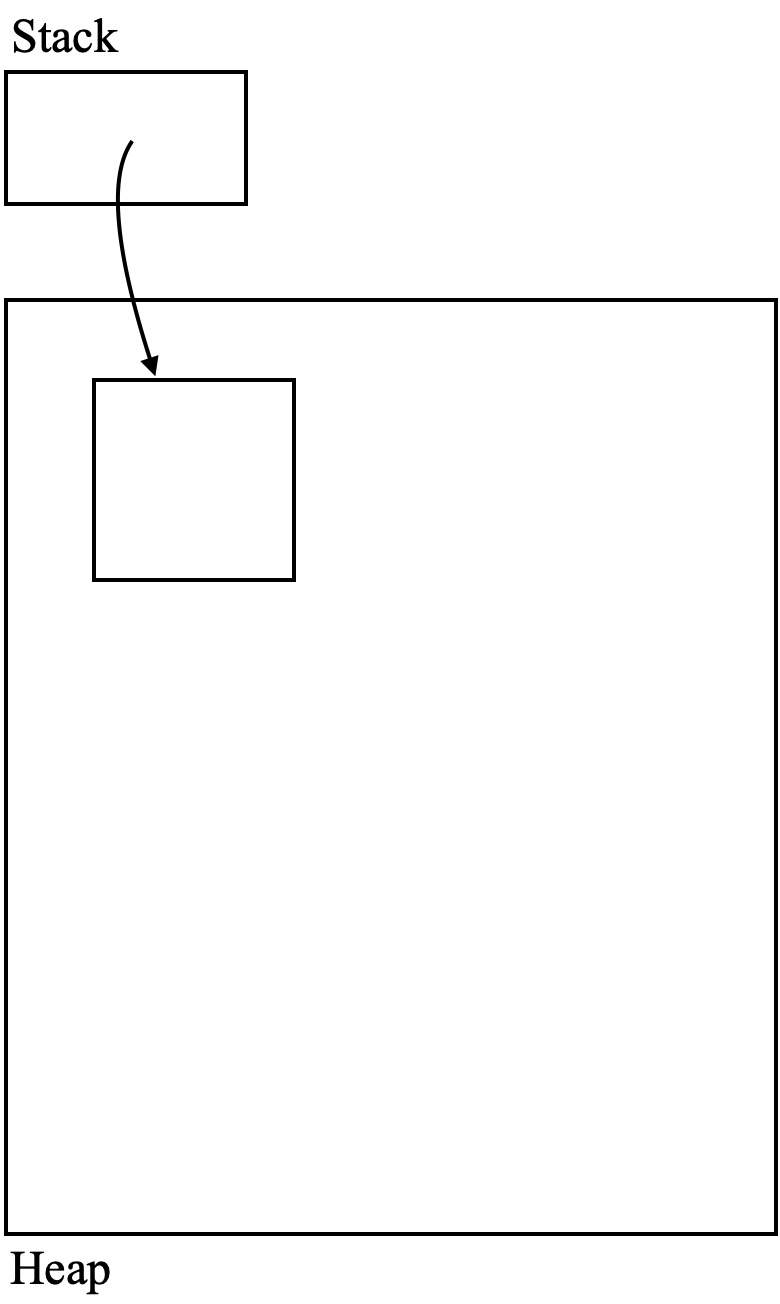
\includegraphics[height=20em]{reachable1}
\end{center}

At this point, \code{C(0)} at \code{0x1000} is reachable because the stack has
the address \code{0x1000}.

After executing \code{a = C(1)}, the memory is as follows:

\begin{center}
\begin{tabular}{cc}
  \begin{tabular}{|c|>{\centering\arraybackslash}p{60pt}|}
    \hline \code{a} & \code{0x1004} \\
    \hline
  \end{tabular}
  &
  \begin{tabular}{|c|>{\centering\arraybackslash}p{60pt}|}
    \hline \code{0x1000} & \code{C(0)} \\
    \hline \code{0x1004} & \code{C(1)} \\
    \hline
  \end{tabular}
  \\ Stack & Heap
\end{tabular}

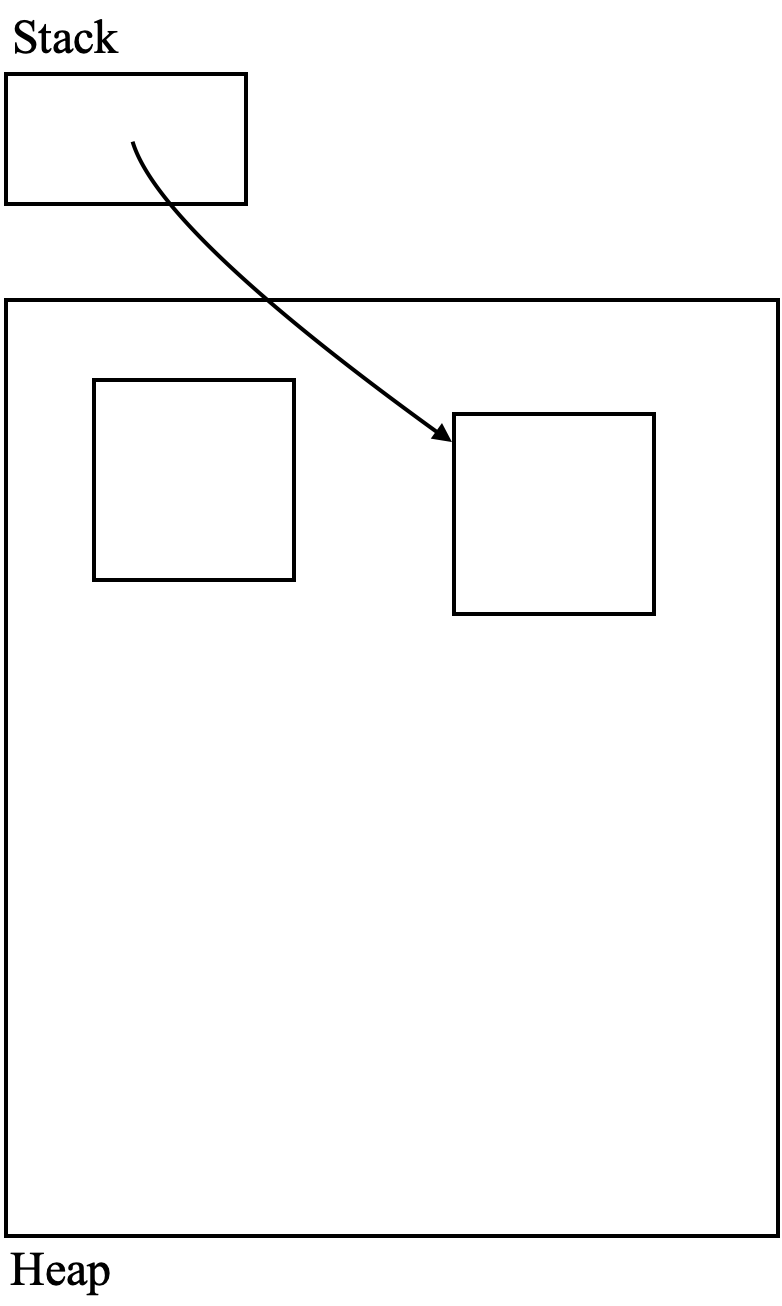
\includegraphics[height=20em]{reachable2}
\end{center}

Now, \code{C(1)} at \code{0x1004} is reachable, but \code{C(0)} at \code{0x1000}
is not reachable any longer.

Note that it is possible that an object is reached in more than one step. For
example, consider the following code:

\begin{verbatim}
case class C(x: C)

var a = C(null)
a = C(a)
\end{verbatim}

After executing the program, the memory is as follows:

\begin{center}
\begin{tabular}{cc}
  \begin{tabular}{|c|>{\centering\arraybackslash}p{60pt}|}
    \hline \code{a} & \code{0x1004} \\
    \hline
  \end{tabular}
  &
  \begin{tabular}{|c|>{\centering\arraybackslash}p{60pt}|}
    \hline \code{0x1000} & \code{C(null)} \\
    \hline \code{0x1004} & \code{C(0x1000)} \\
    \hline
  \end{tabular}
  \\ Stack & Heap
\end{tabular}

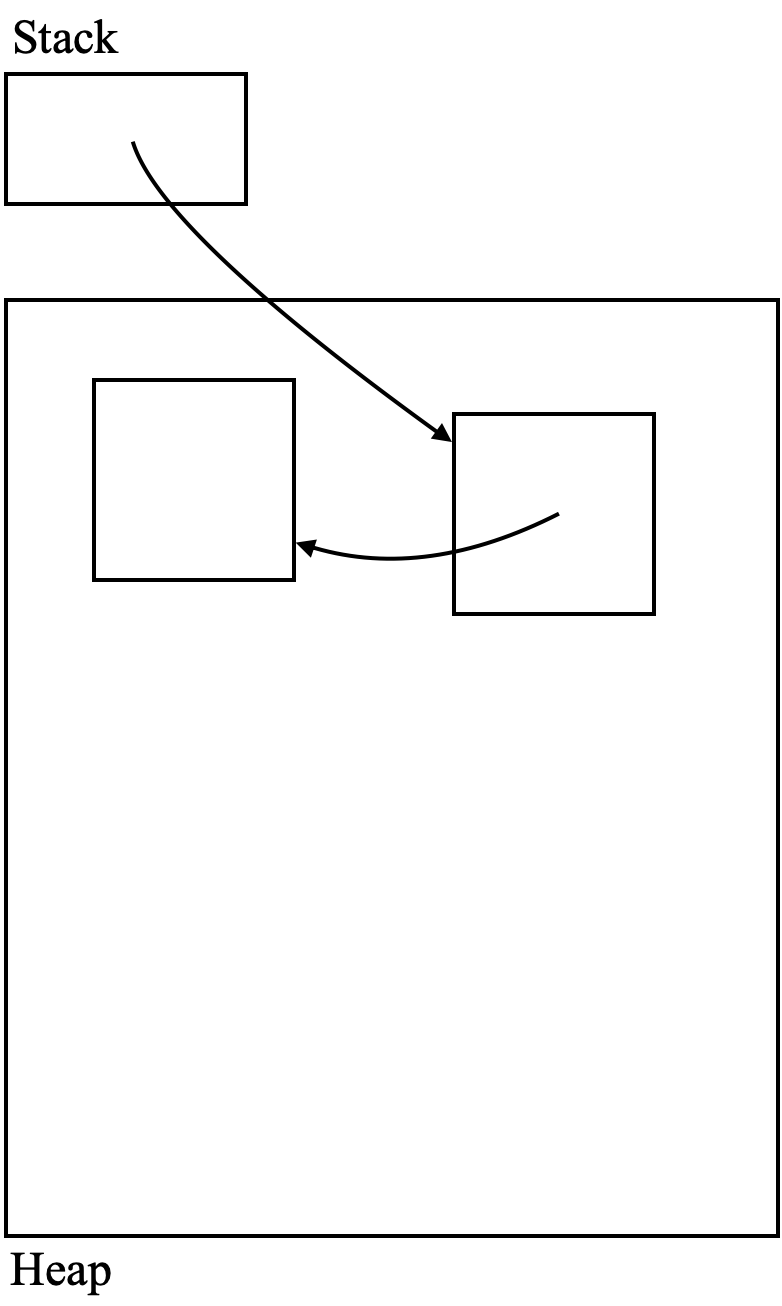
\includegraphics[height=20em]{reachable3}
\end{center}

Although the stack does not contain \code{0x1000}, \code{C(null)} at
\code{0x1000} is still reachable because the stack has \code{0x1004} and
\code{0x1000} is stored at the address \code{0x1004}.

The intuition of GC is that unreachable objects cannot be used by programs. The
stack stores the values of local variables. Therefore, programs can access any
values on the stack by reading local variables. However, objects on the heap do
not directly correspond to specific program constructs. To access them, programs
need to read their addresses from somewhere. It implies that programs can access
objects only when they are reachable from the stack\sidenote{More precisely,
objects reachable from the stack and \textit{registers}\index{register} are
accessible. Registers are small memory storage inside the CPU. They also are
used to store the values of local variables. Sometimes, the stack and registers
are collectively called the \textit{root}\index{root} in the context of GC. For
simplicity, this book ignores registers.} by following pointers.

Both of the above examples advocate this intuition. In the first example, after
executing \code{var a = C(0)}, \code{C(0)} is reachable. The object is indeed
accessible by reading the variable \code{a}. Then, after executing \code{a =
C(1)}, \code{C(0)} becomes unreachable and inaccessible; reading \code{a}
accesses \code{C(1)}, not \code{C(0)}. In the second example, \code{C(null)} is
reachable even after executing \code{a = C(a)}, and the program can access
\code{C(null)} by reading \code{a.x}.

Following this intuition, GC finds unreachable objects and deallocates them
during the execution of programs. In this way, GC never makes dangling pointers.
It is guaranteed that all the deallocated objects are garbage. In other words,
GC completely prevents UAF.

However, GC cannot completely prevents memory leaks. It is because not every
garbage is unreachable. Consider the following code:

\begin{verbatim}
case class C(x: Int)

val a = C(0)
... // never use `a`
\end{verbatim}

The program creates \code{C(0)} but never uses it. In this case, \code{C(0)} is
garbage but reachable. Since \code{C(0)} is reachable, GC never deallocates it
although it is garbage in fact. Therefore, this causes a memory leak.
Fortunately, code like the above is rare in practice. For this reason, memory
leaks caused by GC are usually negligible.

Note that not every automatic memory management uses GC; for example, the Rust
compiler analyzes programs and automatically inserts \code{drop} at compile
time. It is different from GC, which operates at run time. Although GC is not
the only way of achieving automatic memory management, GC is still the most
popular one.

The remainder of the chapter introduces three widely-used techniques to
implement GC.

\section{Reference Counting}

Under reference counting, each object is accompanied by a reference count. The
reference count of an object is an integer representing the number of pointers
referring the object. When an object is created, its reference count equals
zero. Each time a pointer to the object is created, the reference count
increases by one, and each time a pointer to the object is destroyed, the
reference count decreases by one. When the reference count becomes zero after a
decrement, the object is considered unreachable and immediately deallocated.

Consider the following code:

\begin{verbatim}
case class C(var x: Any)

var a = C(0)
val b = C(a)
a = C(1)
b.x = a
\end{verbatim}

Let us see how reference counting collects garbage with the example.

After executing \code{var a = C(0)}, the memory is as follows:

\begin{center}
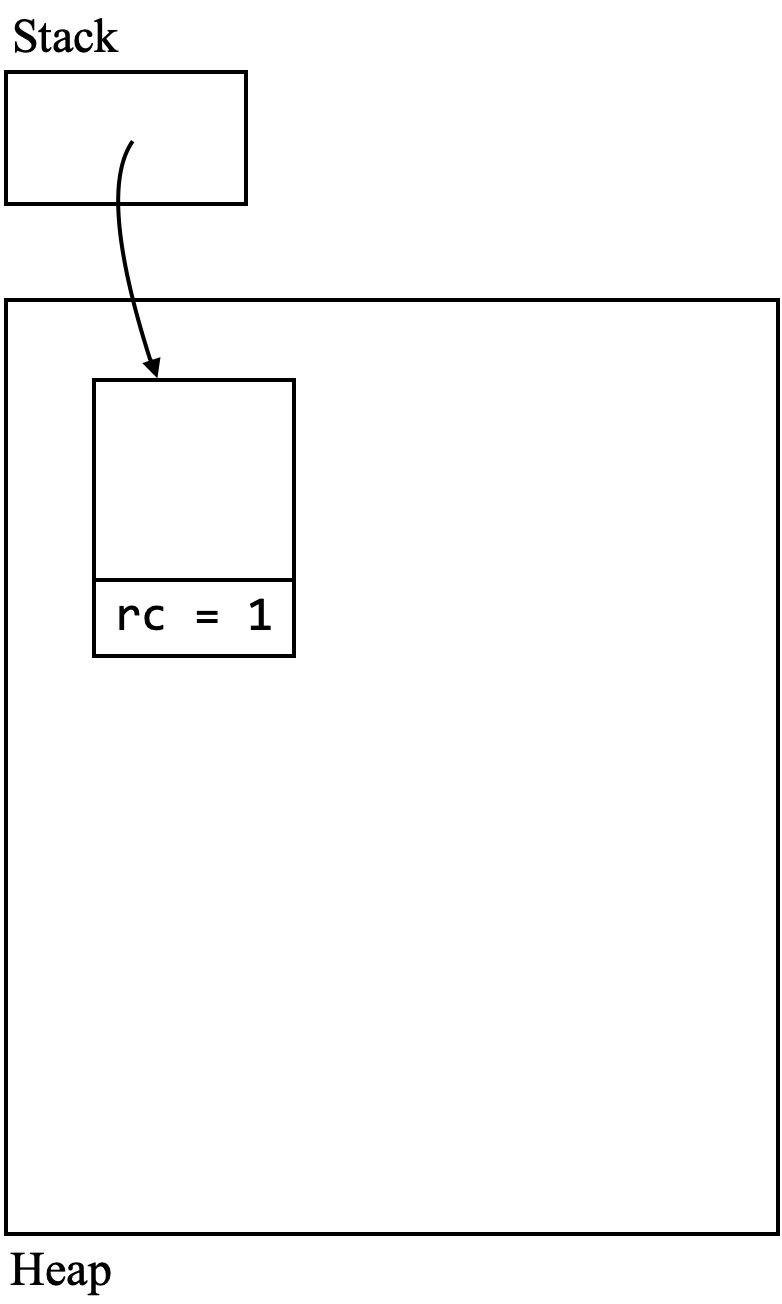
\includegraphics[height=20em]{rc1}
\end{center}

The reference count of \code{C(0)} increases from \code{0} to \code{1}
because a pointer to the object has been created and stored in the variable
\code{a} on the stack.

After executing \code{val b = C(a)}, the memory is as follows:

\begin{center}
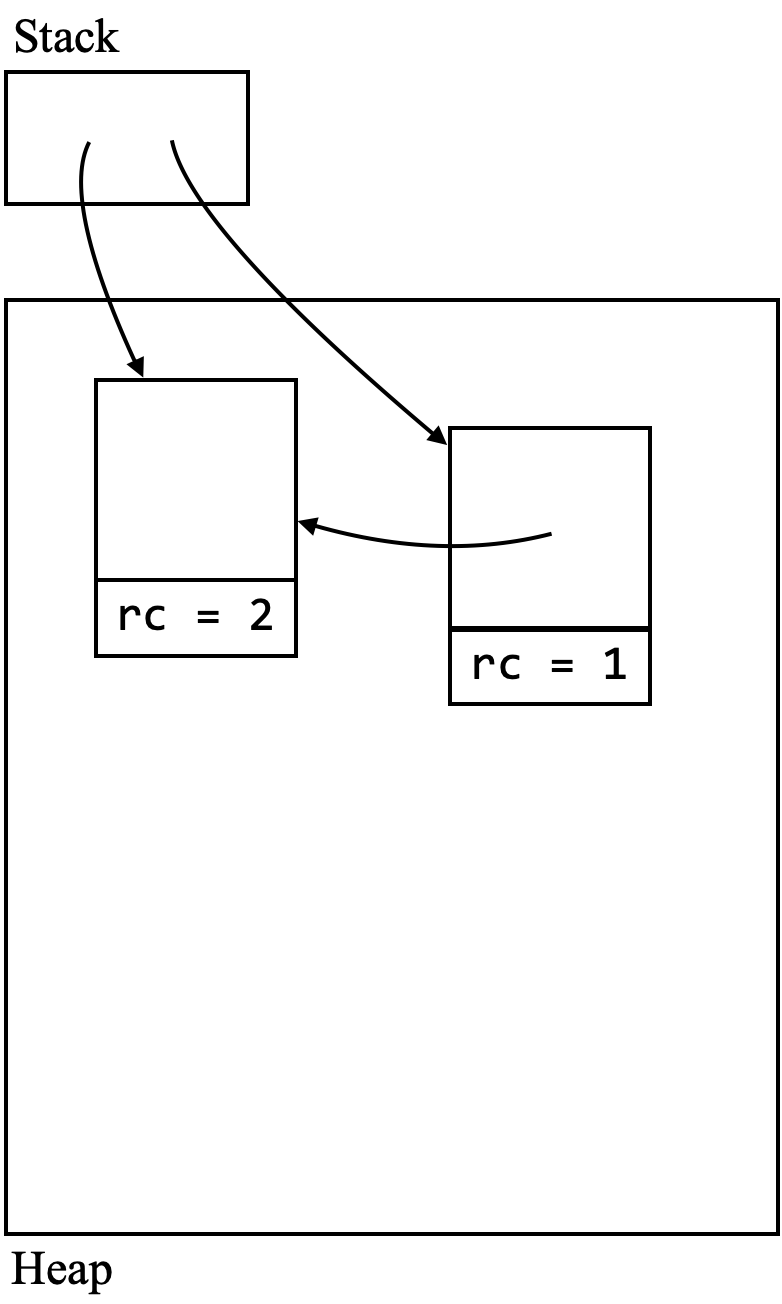
\includegraphics[height=20em]{rc2}
\end{center}

The reference count of \code{C(0)} increases again from \code{1} to \code{2}
because a pointer to the object has been created and stored in \code{C(a)}.

After executing \code{a = C(1)}, the memory is as follows:

\begin{center}
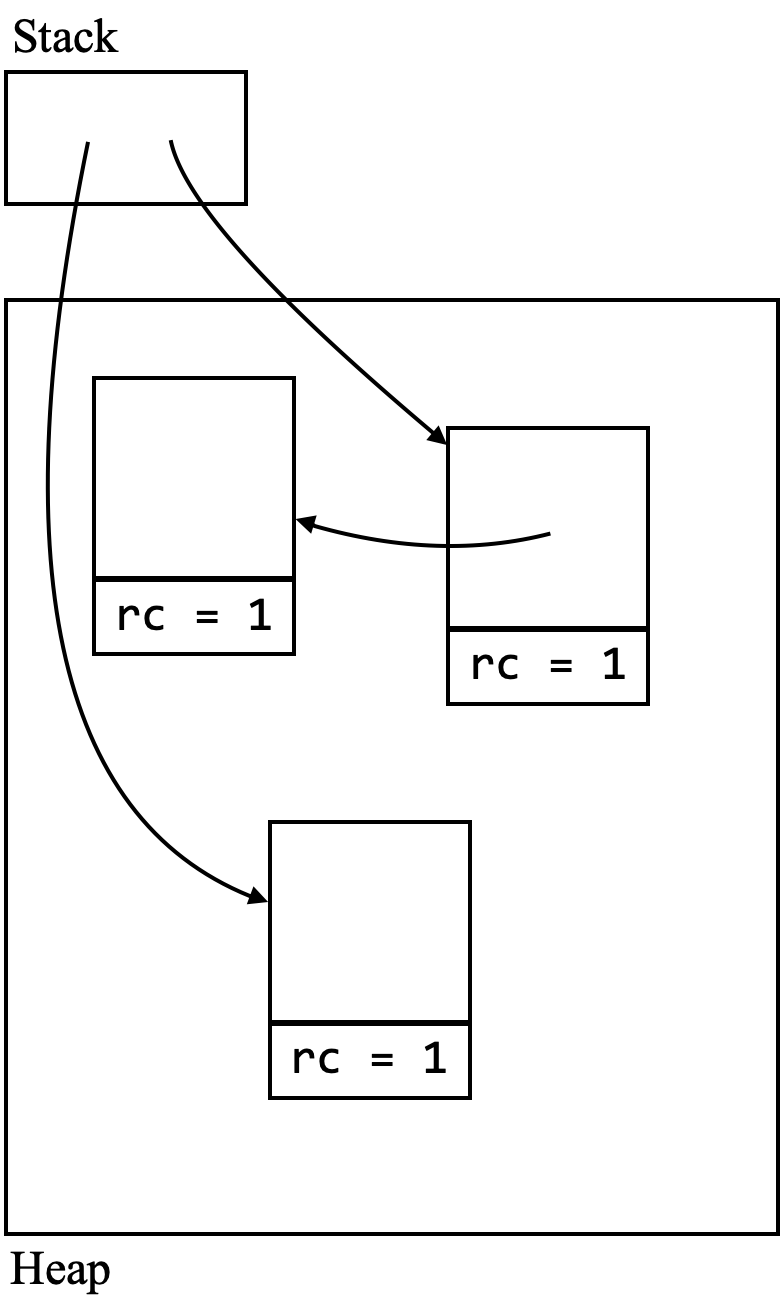
\includegraphics[height=20em]{rc3}
\end{center}

The reference count of \code{C(0)} decreases from \code{2} to \code{1}
because the pointer held by \code{a} has been destroyed. Now, \code{a} has a
pointer to \code{C(1)}.

After executing \code{b.x = a}, the memory is as follows:

\begin{center}
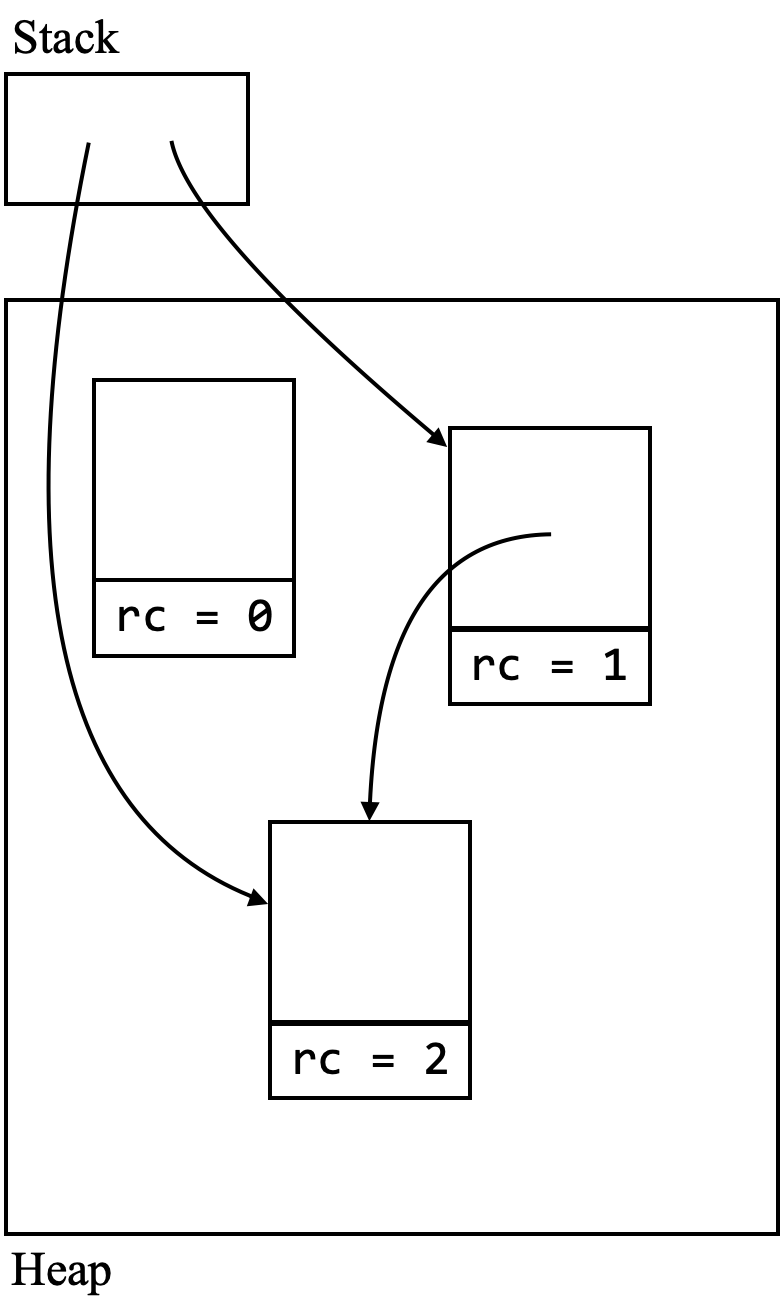
\includegraphics[height=20em]{rc4}
\end{center}

The reference count of \code{C(0)} decreases again from \code{1} to \code{0}
because the pointer held by \code{C(a)} also has been destroyed. Since the
reference count equals zero, the object is considered unreachable and becomes
deallocated.

\begin{center}
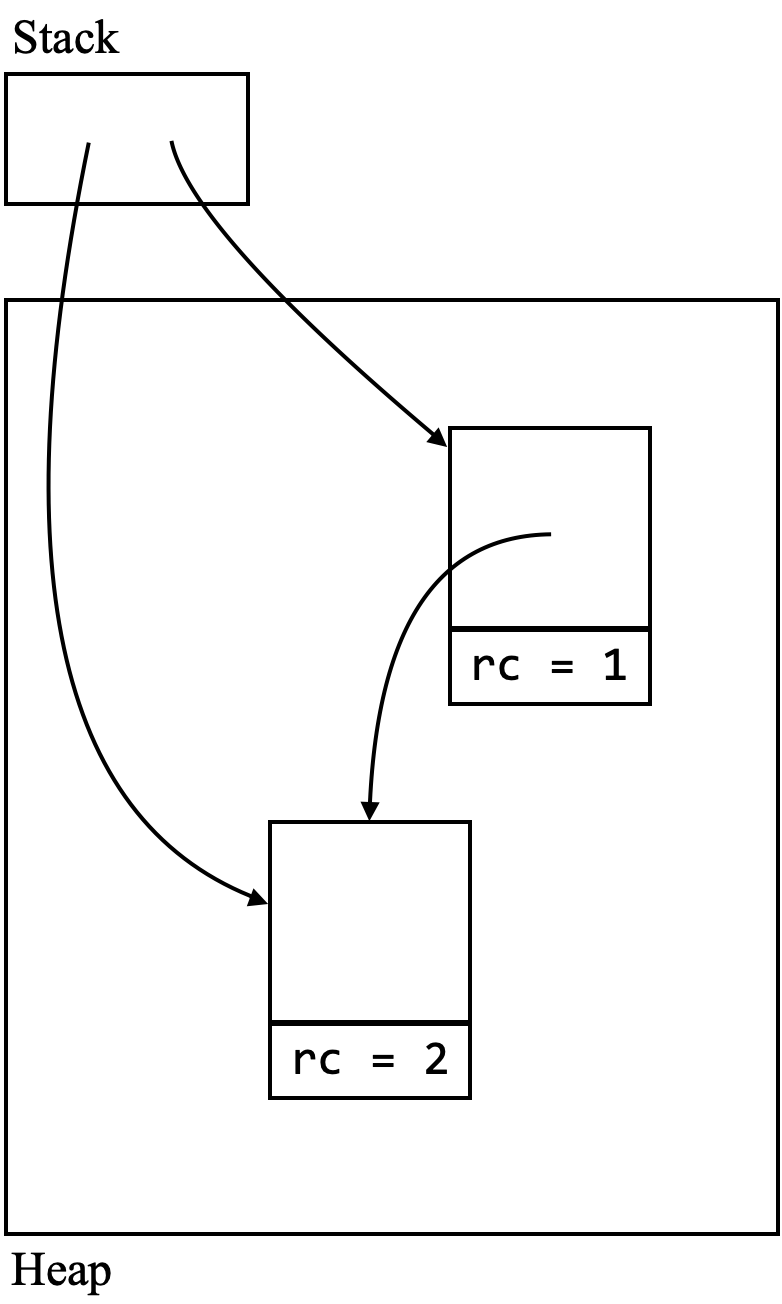
\includegraphics[height=20em]{rc5}
\end{center}

\subsection{Pros}

Reference counting has the following strengths:

\begin{itemize}
  \item It is easy to implement.
  \item Memory reclamation is immediate and takes a short time.
\end{itemize}

\paragraph{Ease of Implementation}

Reference counting requires only reference counts attached to objects
and modification of them at the creation and deletion of pointers. It is
easy to implement; it can be implemented even as a library, without any
language-level support. For example,
\verb!shared_ptr!\sidenote{\url{https://en.cppreference.com/w/cpp/memory/shared_ptr}}
in C++ and
\code{Rc}\sidenote{\url{https://doc.rust-lang.org/std/rc/struct.Rc.html}} in
Rust are well-known library implementations of reference counting.

\paragraph{Immediate Reclamation}

The reference count of an object decreases to zero as soon as it becomes
unreachable. Then, the object is deallocated immediately. Therefore, memory
reclamation is immediate if one uses reference counting. There is little space
wasted in the heap. In addition, checking whether a certain reference count is
zero or not is extremely fast, so the execution of a program never pauses for a
long time due to GC.

\subsection{Cons}

Reference counting has the following weaknesses:

\begin{itemize}
  \item It cannot handle cyclic structures.
  \item Maintaining reference counts takes cost.
  \item It requires free lists.
  \item It suffers from external fragmentation.
\end{itemize}

\paragraph{Cyclic Structure}

Unfortunately, reference counting suffers from memory leaks when objects form
cycles. Consider the following code:

\begin{verbatim}
def f() = {
  val a = C(null)
  val b = C(a)
  a.x = b
}
\end{verbatim}

Suppose that \code{f} is called. After executing \code{val a = C(null)}, the
memory is as follows:

\begin{center}
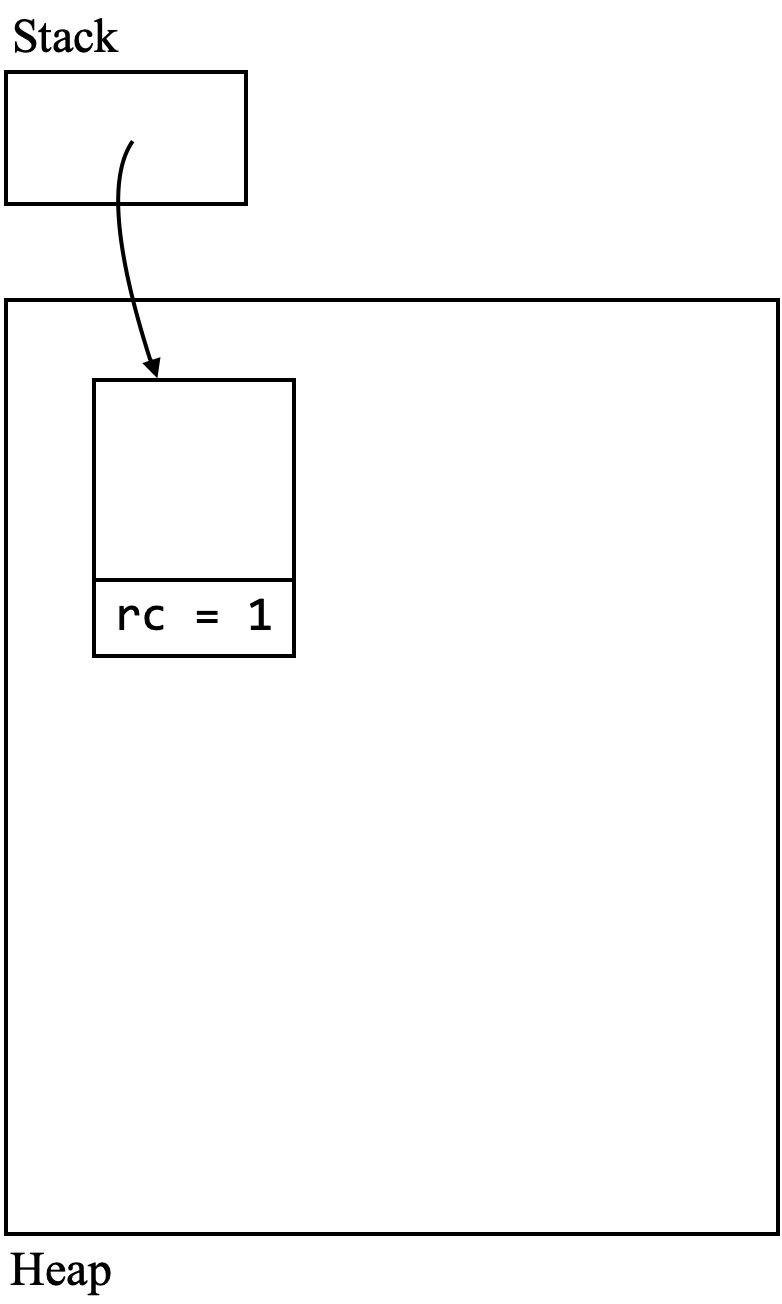
\includegraphics[height=20em]{cycle1}
\end{center}

After executing \code{val b = C(a)}, the memory is as follows:

\begin{center}
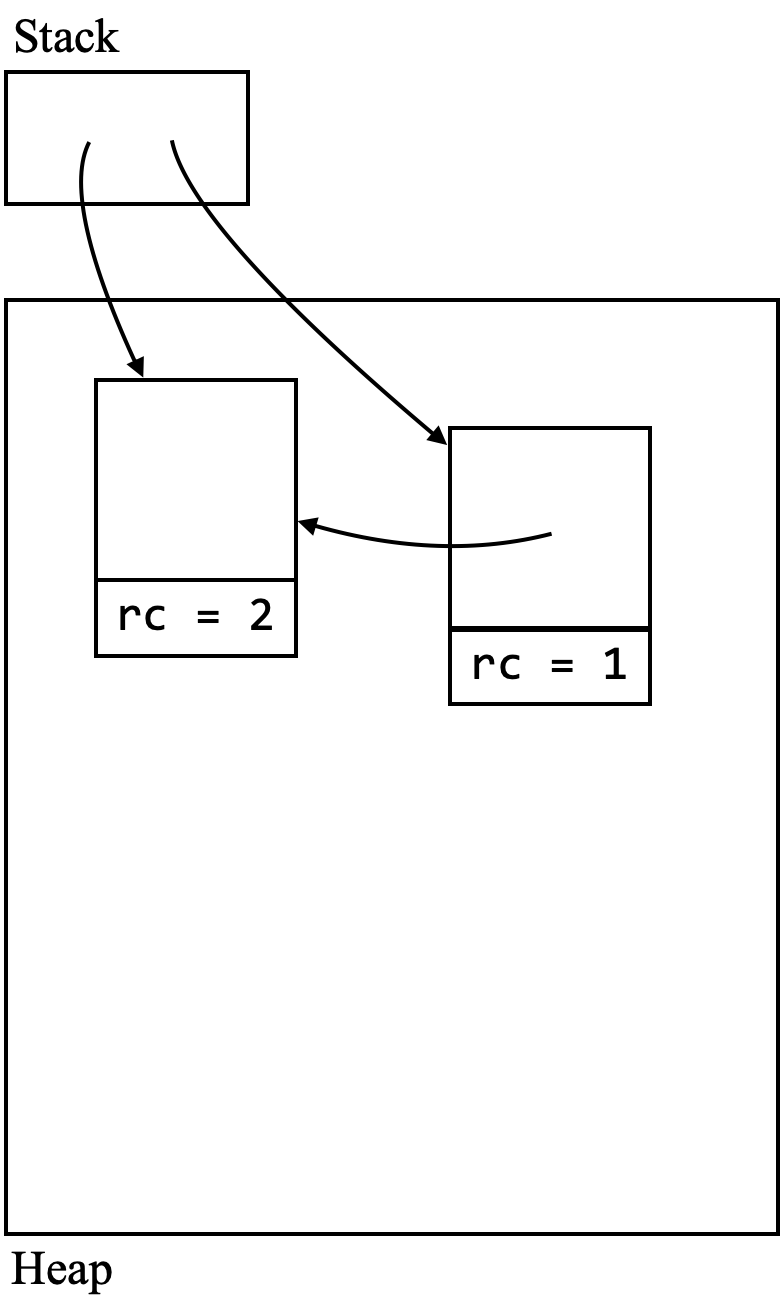
\includegraphics[height=20em]{cycle2}
\end{center}

After executing \code{a.x = b}, the memory is as follows:

\begin{center}
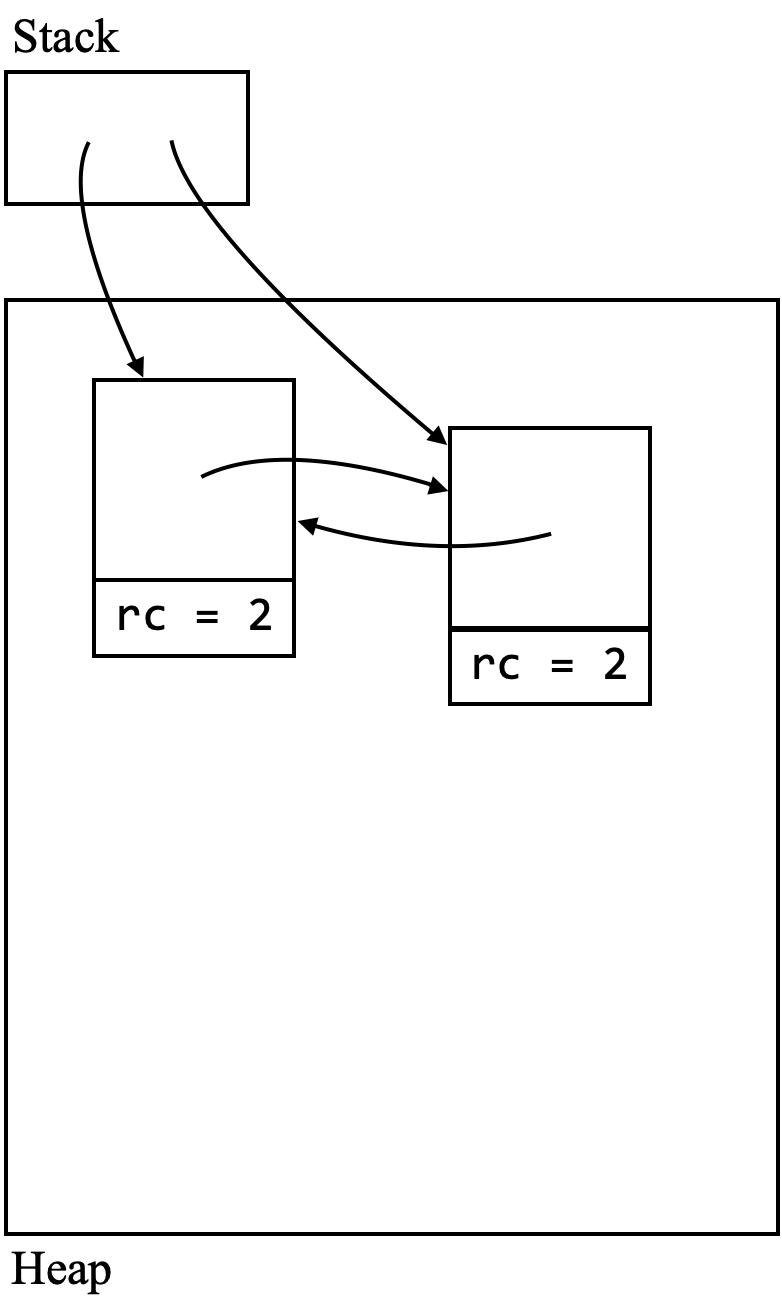
\includegraphics[height=20em]{cycle3}
\end{center}

Each object has a pointer to the other, so a cycle has been formed.

Finally, the function returns. Then, the memory is as follows:

\begin{center}
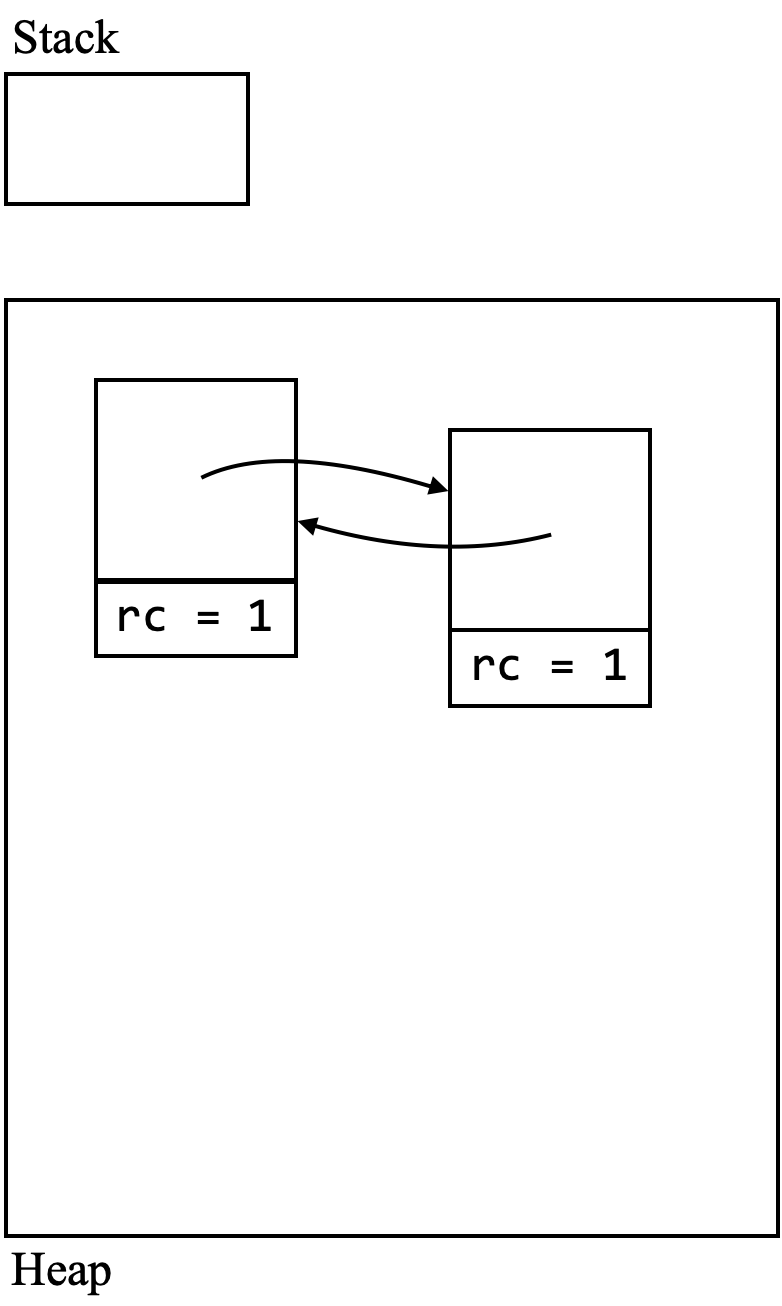
\includegraphics[height=20em]{cycle4}
\end{center}

Both of the local variables \code{a} and \code{b} have been popped off from the
stack, so each of the objects loses one pointer. Therefore, their reference
counts decrease to \code{1}. Since there is no way to reach them from the stack,
they are unreachable. However, their reference counts are not zero. They will
not be deallocated forever. This is definitely a memory leak, and the reason is
the cyclic structure made by the objects.

While the other weaknesses of reference counting cause only performance
degradation, memory leaks due to the inability to handle cyclic structures are a
critical drawback of reference counting. For this reason, reference counting is
often criticized. However, some languages use reference counting despite this
crucial limitation. For example, Python and Swift use reference counting. Each
of them has its own solution to overcome the limitation of reference counting.
Python provides a secondary GC algorithm, which can properly handle cycles,
while having reference counting as the primary
one.\sidenote{\url{https://docs.python.org/3/library/gc.html}} Swift allows
programmers to create \textit{weak references}\index{weak reference}, which are
pointers that do not increase reference counts, in addition to usual pointers,
i.e., \textit{strong references}\index{strong
reference}.\sidenote{\url{https://docs.swift.org/swift-book/LanguageGuide/AutomaticReferenceCounting.html}}
Programmers can use weak references when they want to create cycles without
memory leaks.

\paragraph{Maintaining Reference Counts}

Reference counts occupy some of the heap space. It decreases the total size of
objects that can be allocated on the heap.

In addition, creation and deletion of a pointer always modify reference counts,
which takes some time. It harms the performance of programs compared to other GC
techniques, which modify the heap only when allocating and deallocating
objects, but not when creating and destroying pointers. Note that each object is
allocated and deallocated only once, but pointers to each object can be created
and destroyed multiple times.

\paragraph{Free List}

The free space of the heap is initially a single continuous block of memory.

\begin{center}
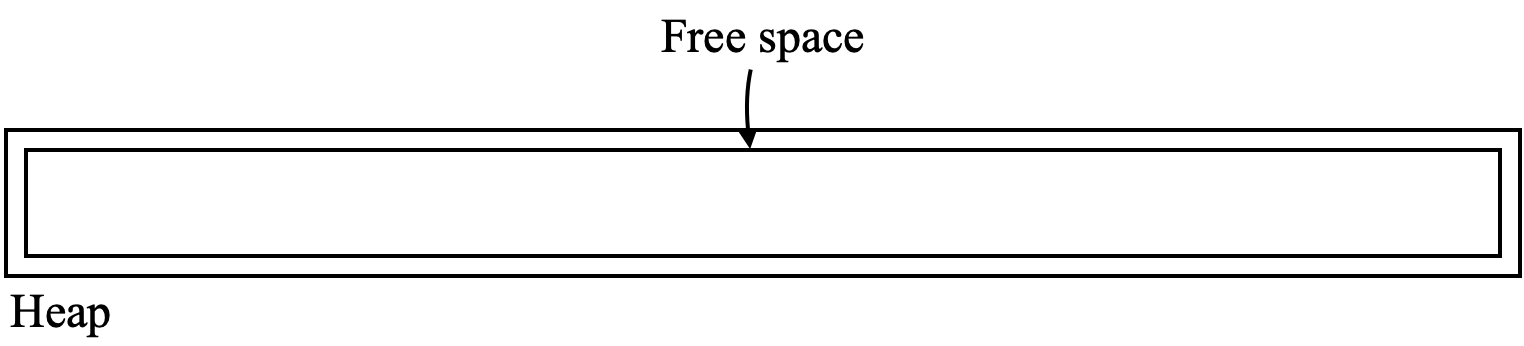
\includegraphics[height=5em]{freelist1}
\end{center}

At this moment, it is enough to know the starting address of the free space to
decide the address of a new allocation.

\begin{center}
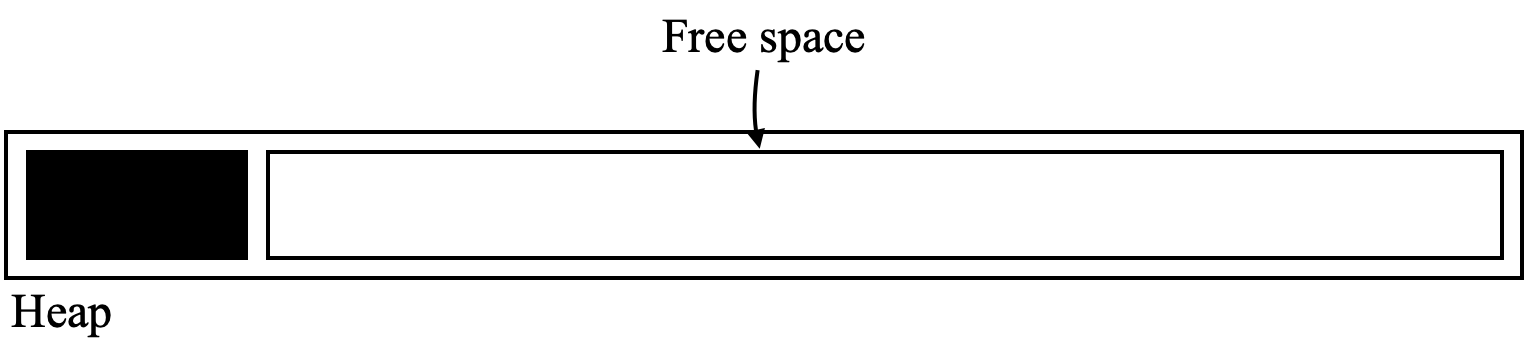
\includegraphics[height=5em]{freelist2}
\end{center}

If there is no garbage and only allocations happen, this remains the same.

\begin{center}
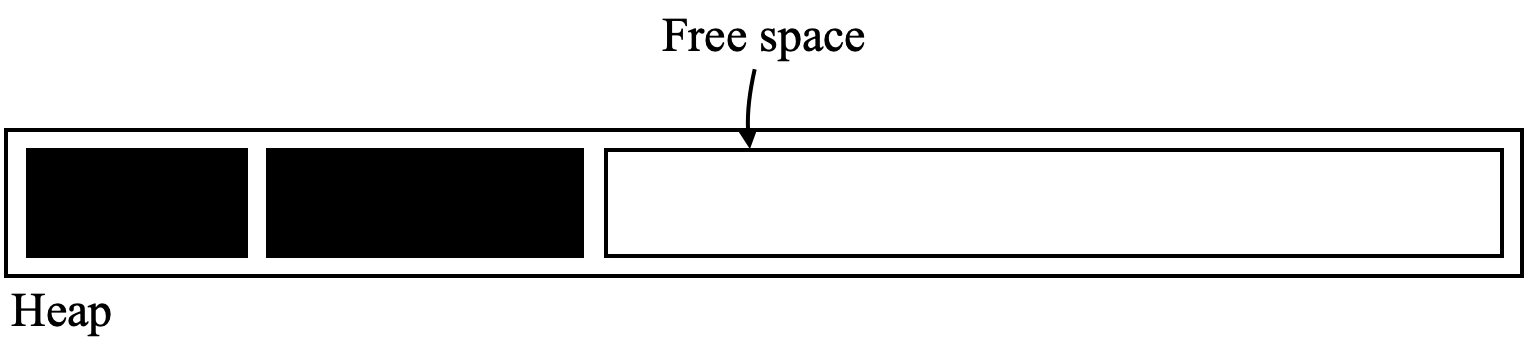
\includegraphics[height=5em]{freelist3}
\end{center}

However, after deallocating some objects, the free space splits into multiple
separated blocks.

\begin{center}
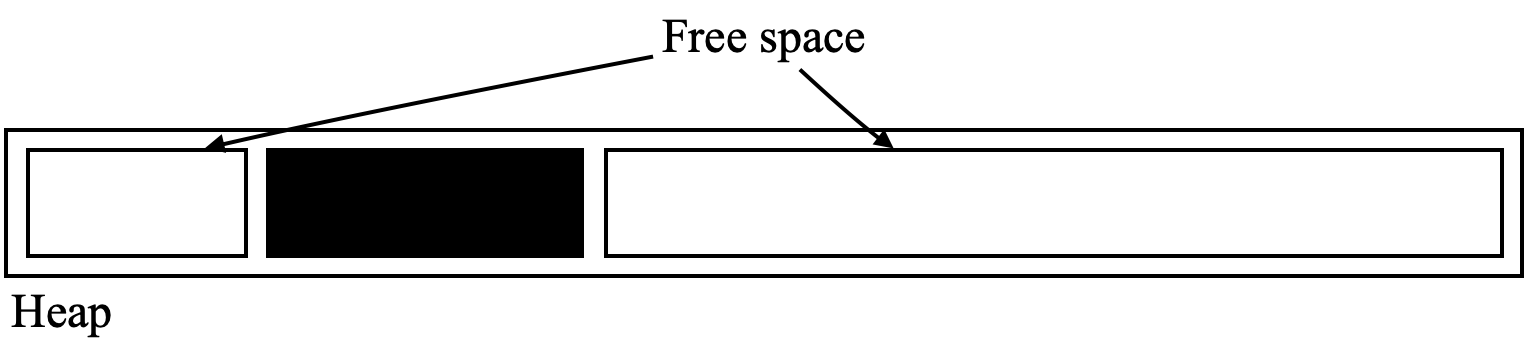
\includegraphics[height=5em]{freelist4}
\end{center}

Therefore, it is not enough to know only the starting address of the free space
in general. The memory manager should know the starting address and the size of
each free block.

For this purpose, the memory manager maintains a data structure called a
\textit{free list}\index{free list} on the heap. A free list is typically a
linked list containing all the free blocks. Maintaining a free list takes some
time and space. Also, each time allocating an object, the memory manager needs to
traverse its free list to find a free block of a proper size.

\paragraph{External Fragmentation}

As mentioned above, the free space splits into multiple blocks. It is called
\textit{external fragmentation}\index{external fragmentation}.  Because of
external fragmentation, an object may not be allocated on the heap although there is
enough free space. Consider the following program:

\begin{enumerate}
  \item allocates four 1KiB-large objects
  \item deallocates the first and the last objects
  \item allocates a 2KiB-large object
\end{enumerate}

Suppose that the program runs with the heap of 4KiB. Ignoring the space for
the reference counts and the free list, the heap after the first four
allocations is as follows:

\begin{center}
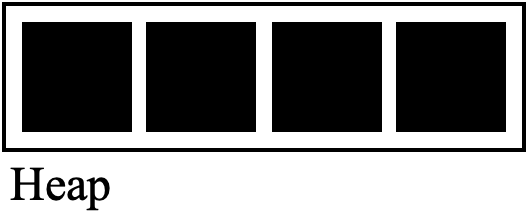
\includegraphics[height=3.5em]{fragmentation1}
\end{center}

After the deallocations, the heap is as follows:

\begin{center}
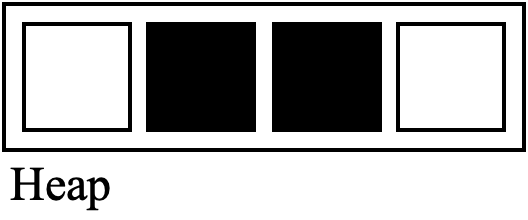
\includegraphics[height=3.5em]{fragmentation2}
\end{center}

Then, it is impossible to allocate the 2KiB-large object although the heap has
free space of 2KiB.

External fragmentation also harms cache utilization. When allocating multiple
objects to be used together, it is desirable to place them close to each other
in the memory.  When it is achieved, we say that the
\textit{locality}\index{locality} is good.  Good locality is important because
it makes objects go into a single cache block and, thus, reduces cache misses.
However, the locality is usually poor due to external fragmentation. Consider
the following heap:

\begin{center}
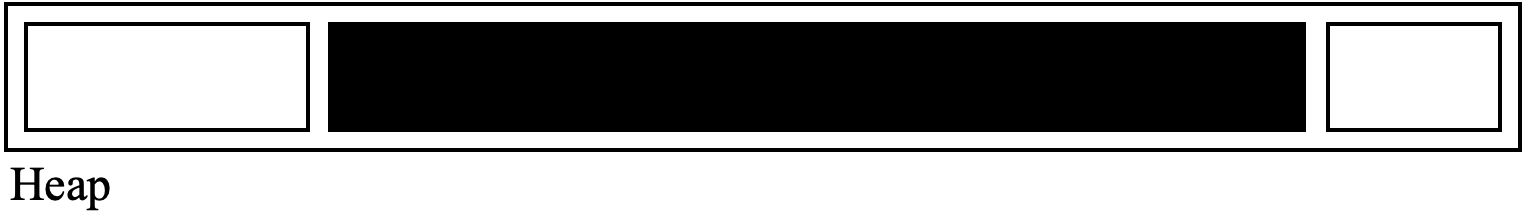
\includegraphics[height=3.5em]{locality1}
\end{center}

If a program allocates two objects, they are placed far away from each other.

\begin{center}
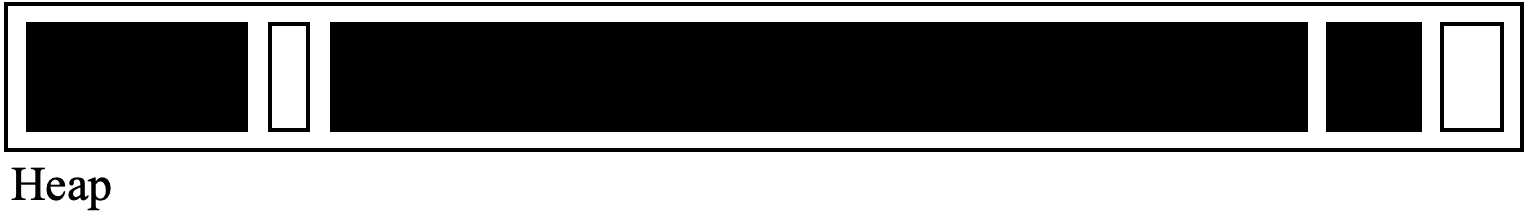
\includegraphics[height=3.5em]{locality2}
\end{center}

\section{Mark-and-Sweep GC}

Unlike reference counting, which possibly deallocates a new unreachable object
each time a pointer is destroyed, \textit{mark-and-sweep
GC}\index{mark-and-sweep garbage collection} finds and deallocates all the
unreachable objects at once only when GC is triggered for some reason (e.g., the
heap is full). Mark-and-sweep GC consists of two phases: the marking phase and
the sweeping phase. The memory manager ``marks'' all the reachable objects in
the marking phase and ``sweeps,'' i.e. deallocates, all the unmarked objects in
the sweeping phase.

\newcommand{\urch}{\textsf{Unreached}\xspace}
\newcommand{\uscn}{\textsf{Unscanned}\xspace}
\newcommand{\scn}{\textsf{Scanned}\xspace}

Let us see how mark-and-sweep GC works in detail. During the marking phase, each
object is in one of the following states:
\begin{itemize}
  \item \urch: This object has not been explored yet. It may be unreachable and is a candidate
    for deallocation. However, the state may change.
  \item \uscn: This object is reachable and will not be deallocated. It has a
    pointer to an \urch object, so a further ``scan'' is required.
  \item \scn: This object is reachable and will not be deallocated. It does not
    have any pointers to \urch objects.
\end{itemize}

When the marking phase starts, all the objects are \urch, which is
represented by a white box.

\begin{center}
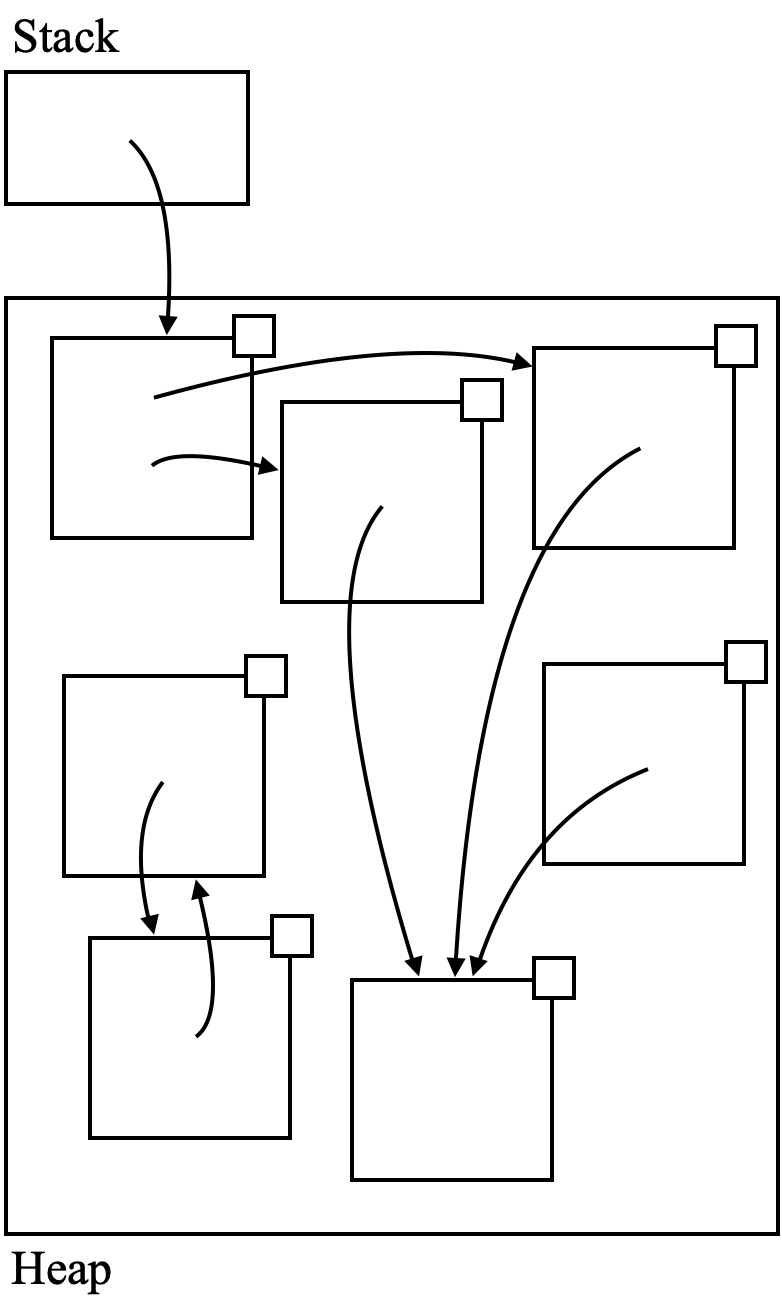
\includegraphics[height=20em]{ms1}
\end{center}

As the first step, objects pointed by on-stack pointers move from the \urch
state to the \uscn state, which is represented by a gray box.

\begin{center}
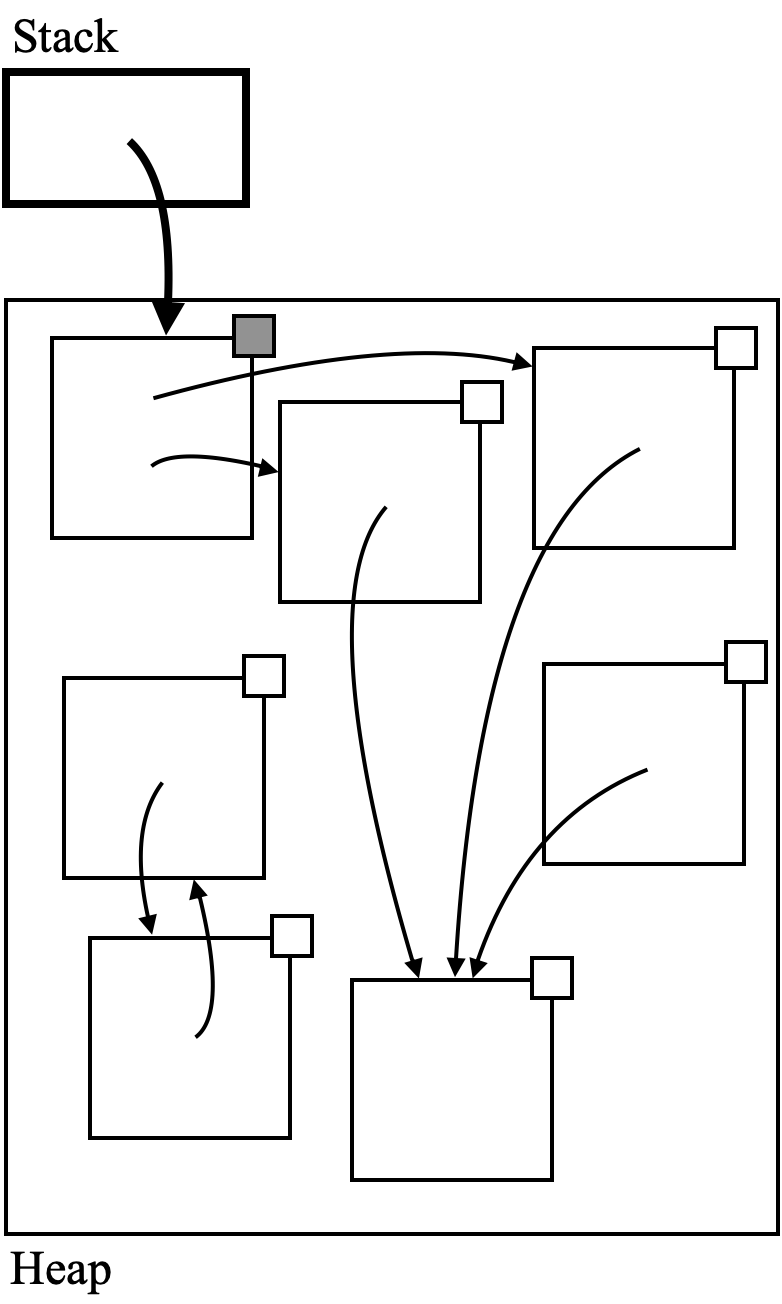
\includegraphics[height=20em]{ms2}
\end{center}

The memory manager chooses one \uscn object and ``scans'' the object by
following all the pointers in the object.  All the \urch objects pointed by the
pointers move to the \uscn state. After the scan, the chosen object becomes
\scn, which is represented by a black box.

\begin{center}
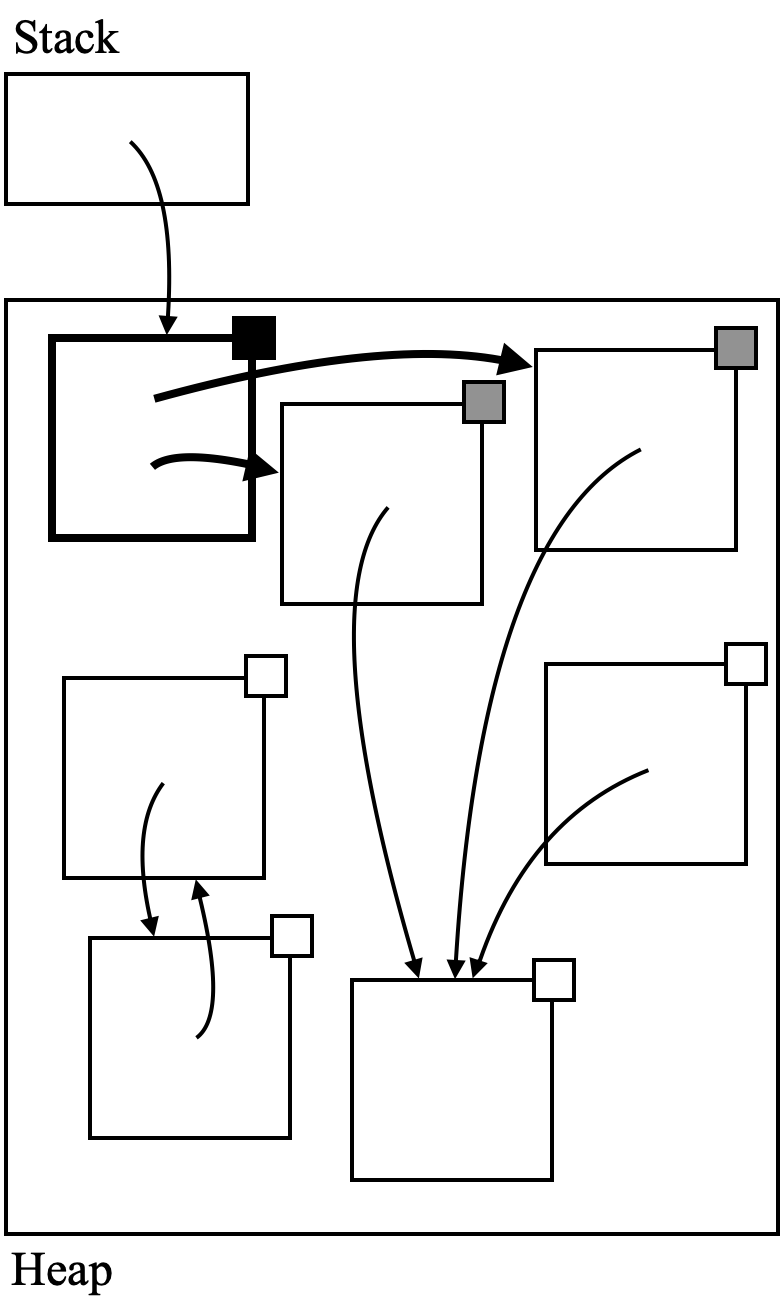
\includegraphics[height=20em]{ms3}
\end{center}

This repeats until there is no \uscn object.

\begin{center}
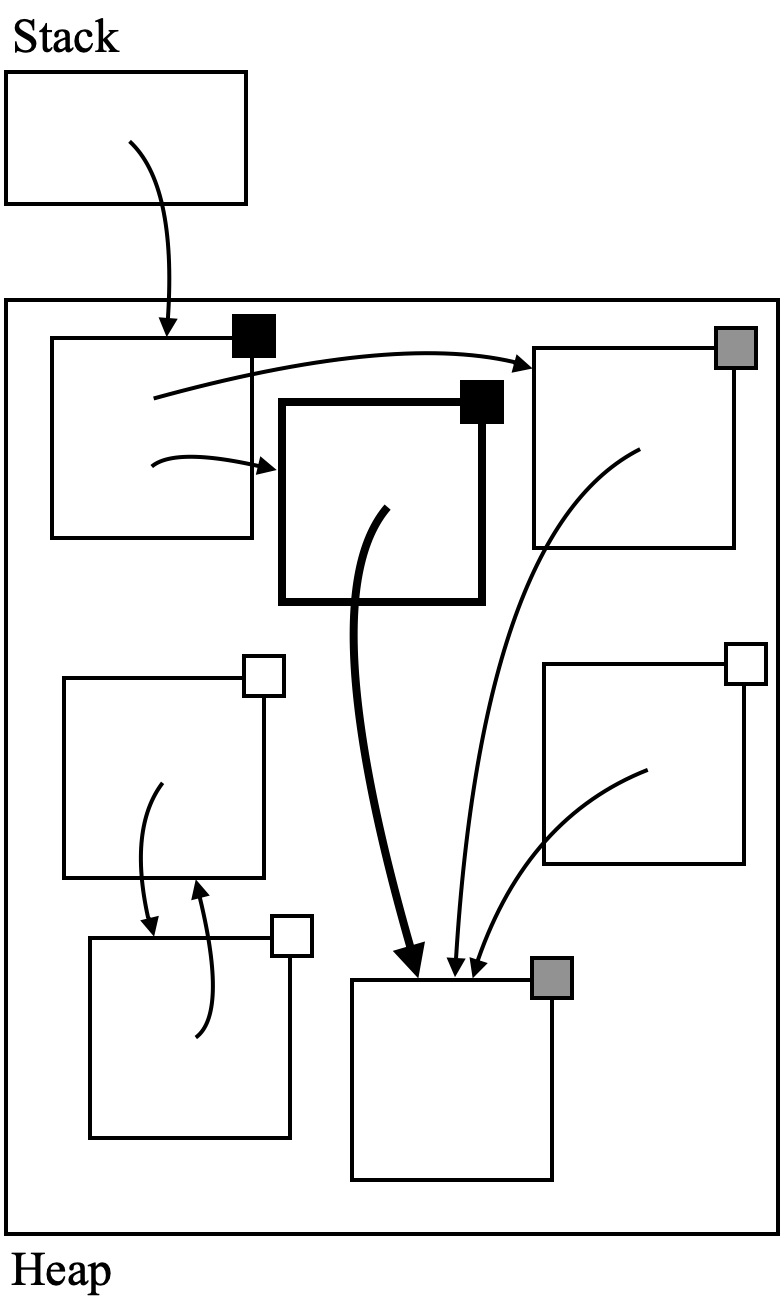
\includegraphics[height=20em]{ms4}

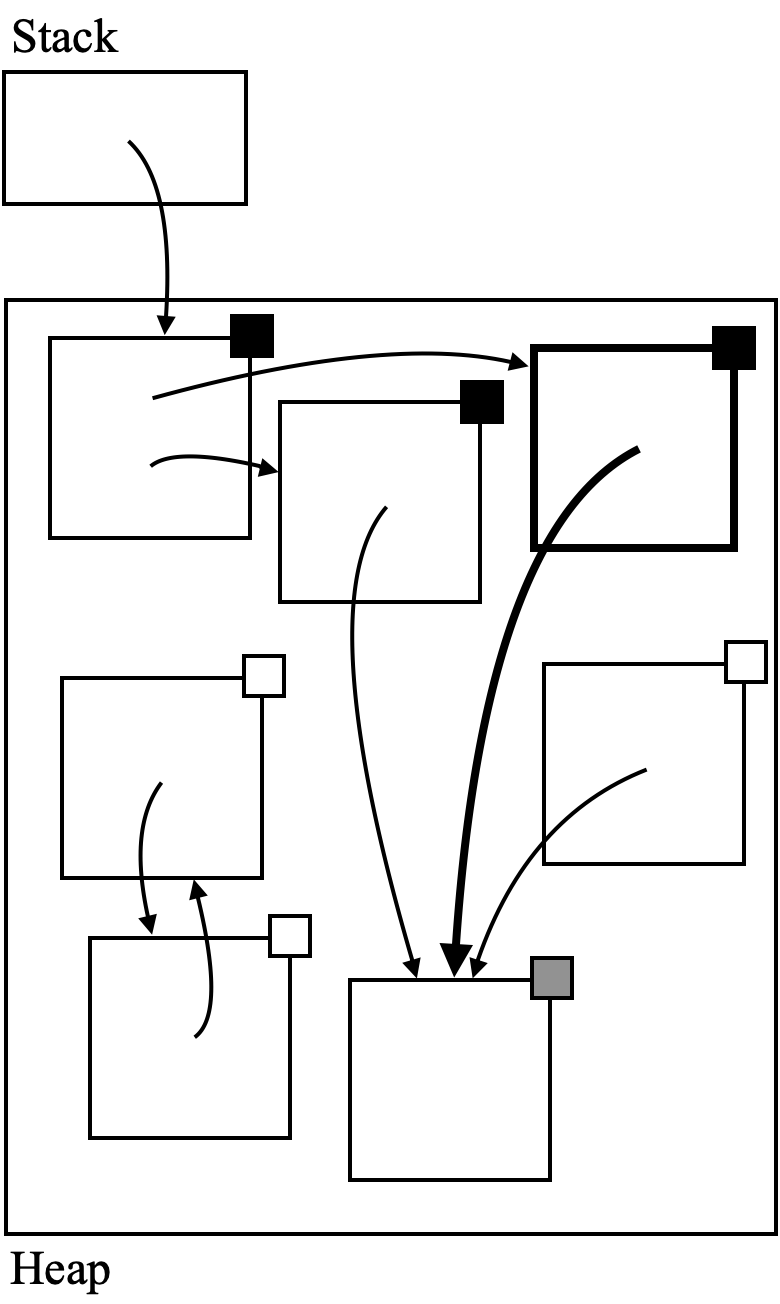
\includegraphics[height=20em]{ms5}

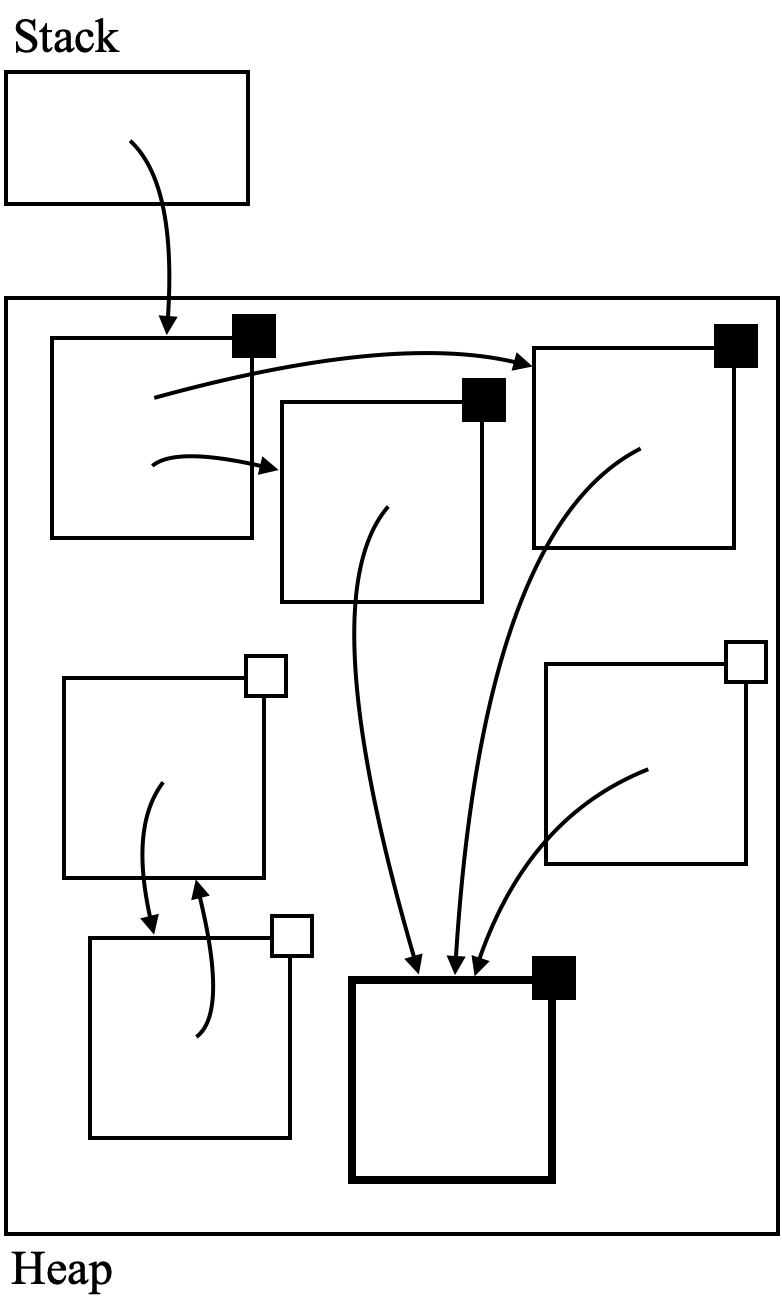
\includegraphics[height=20em]{ms6}
\end{center}

If there is no \uscn object, the marking phase ends.

In the sweeping phase, each object is in either \urch or \scn state.  \scn
objects
are considered marked, and \urch objects are considered unmarked.  Since unmarked
objects are unreachable, all the unmarked objects are deallocated.

\begin{center}
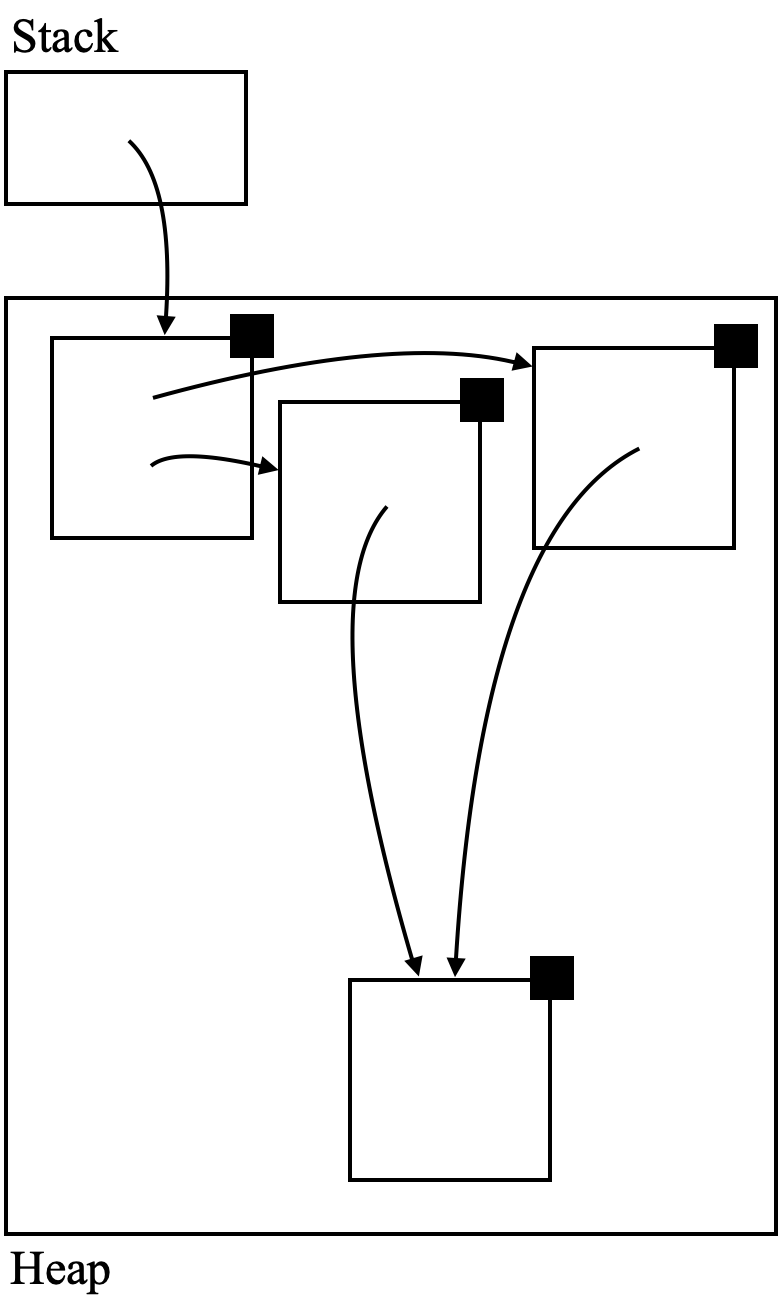
\includegraphics[height=20em]{ms7}
\end{center}

\subsection{Pros}

Unlike reference counting, mark-and-sweep GC can handle cyclic structures.

\subsection{Cons}

Mark-and-sweep GC has the following weaknesses:

\begin{itemize}
  \item It requires free lists.
  \item It suffers from external fragmentation.
  \item Execution pauses during GC.
\end{itemize}

Just like reference counting, mark-and-sweep GC also requires free lists and
suffers from external fragmentation.

\paragraph{Execution Pause}

When GC is triggered, the memory manager scans the entire heap. It takes some
time, especially when the heap is large and has many objects. To correctly decide
the reachability of each object, the execution must stop during GC. Therefore,
a program pauses for a while when GC is triggered. Since programmers cannot
control the exact timing of GC, pauses caused by GC are mostly unpredictable.

To alleviate this issue, modern GC implementations adopt various techniques such
as parallel GC, incremental GC, and concurrent GC, which are beyond the scope of
this book.

\section{Copying GC}

\textit{Copying GC}\index{copying garbage collection} is similar to
mark-and-sweep GC; it finds and deallocates all the unreachable objects when GC
is triggered. However, it copies all the reachable objects and reorganizes them in
a compact layout. For this purpose, it divides the heap into two parts: the
\textit{from-space}\index{from-space} and the \textit{to-space}\index{to-space}.

Every allocation happens in the from-space. Therefore, when GC is triggered,
all the objects are in the from-space, and the to-space is empty.

\begin{center}
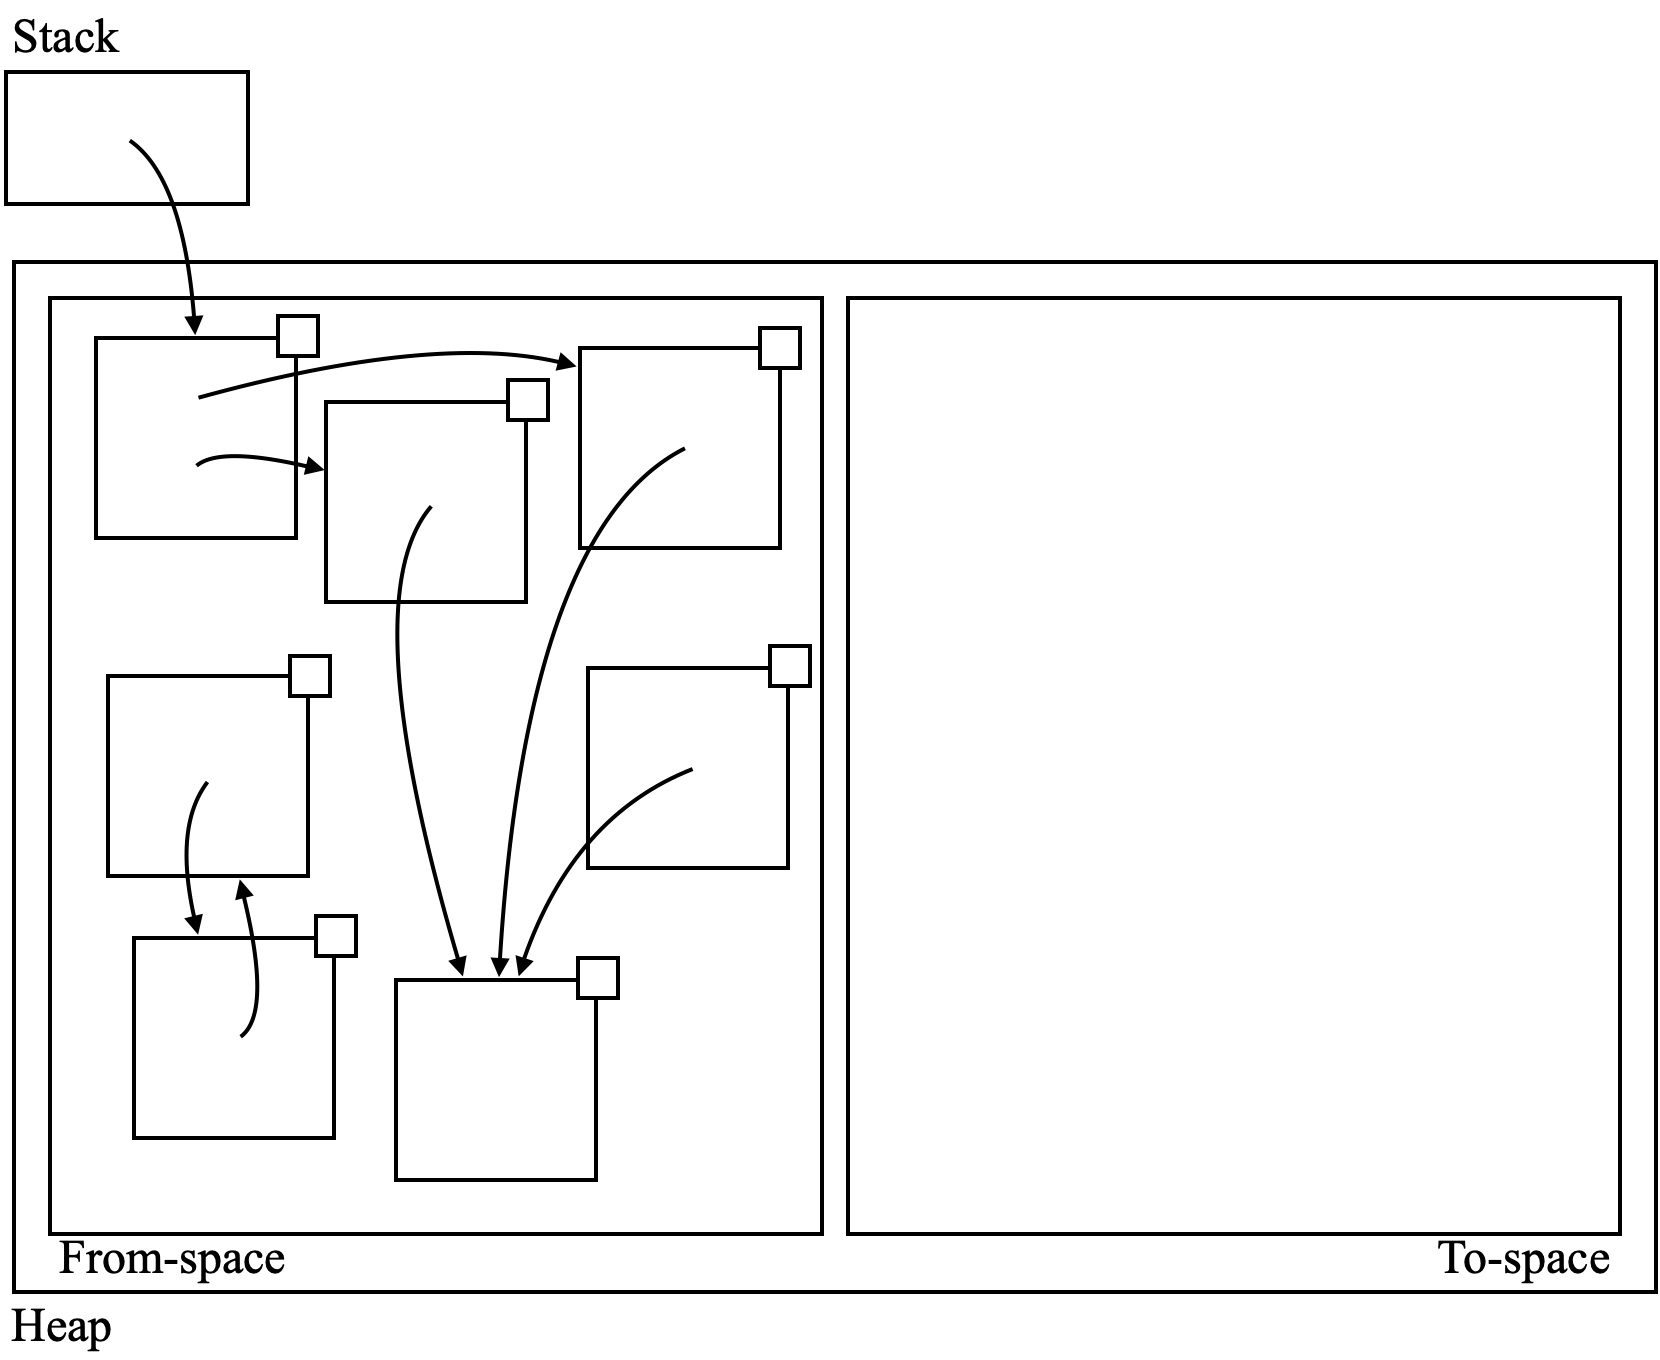
\includegraphics[height=20em]{copying1}
\end{center}

The operation of copying GC is quite similar to the marking phase of
mark-and-sweep GC. It starts from the stack and marks objects reached by following
pointers. The difference is that an object is copied from the from-space to
to-space when it becomes \uscn from \urch. First, all the objects
reachable from the stack in one step are copied to the to-space.

\begin{center}
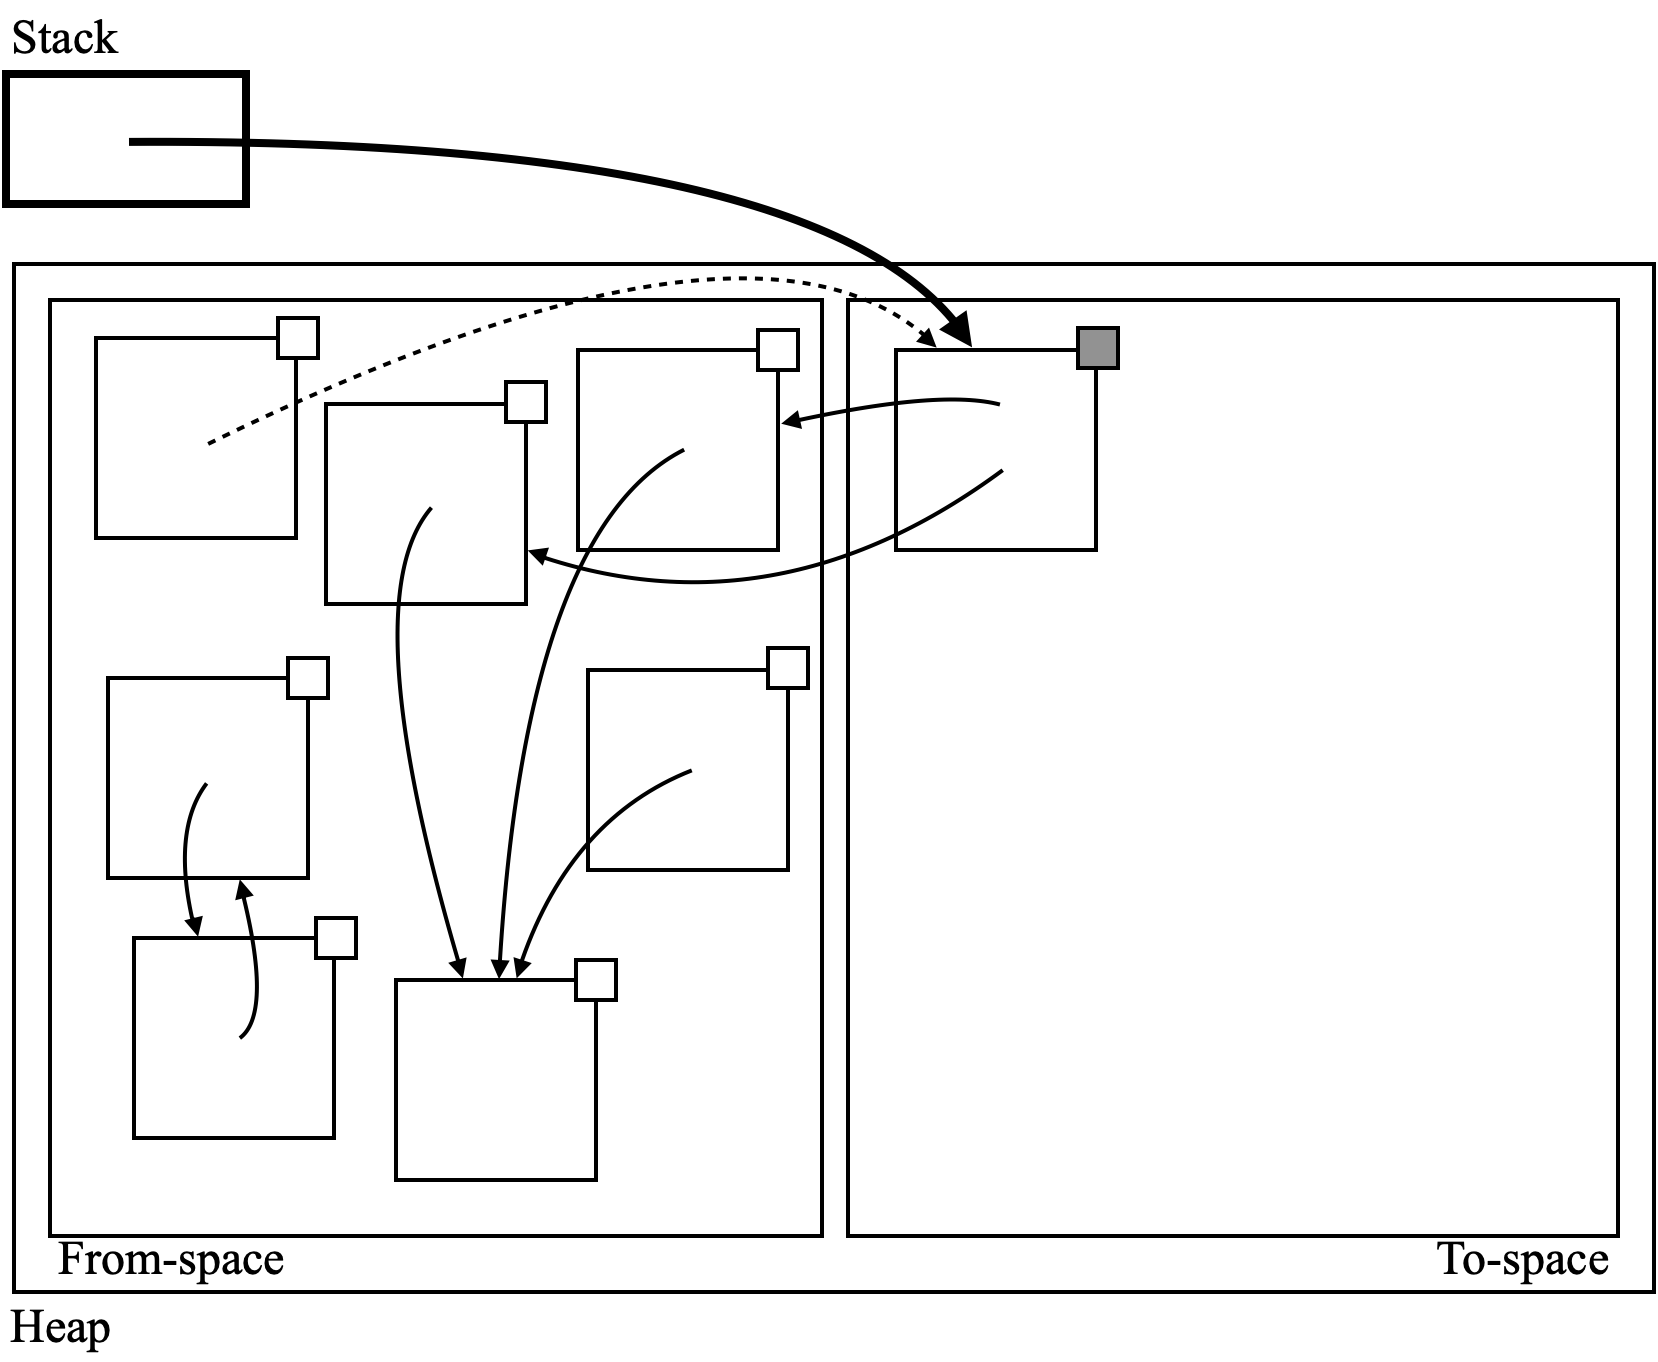
\includegraphics[height=20em]{copying2}
\end{center}

When copying an object, existing pointers to the object are updated so that
they correctly point to the object in the to-space. In addition, a
\textit{forwarding pointer}\index{forwarding pointer} (an arrow with a dashed
line) to the object in the to-space is stored in the object in the from-space.
The forwarding pointer allows the memory manager to correctly update pointers
to be discovered in the future.

The memory manager chooses one \uscn object and makes all the pointed \urch
objects \uscn. The chosen object becomes \scn.

\begin{center}
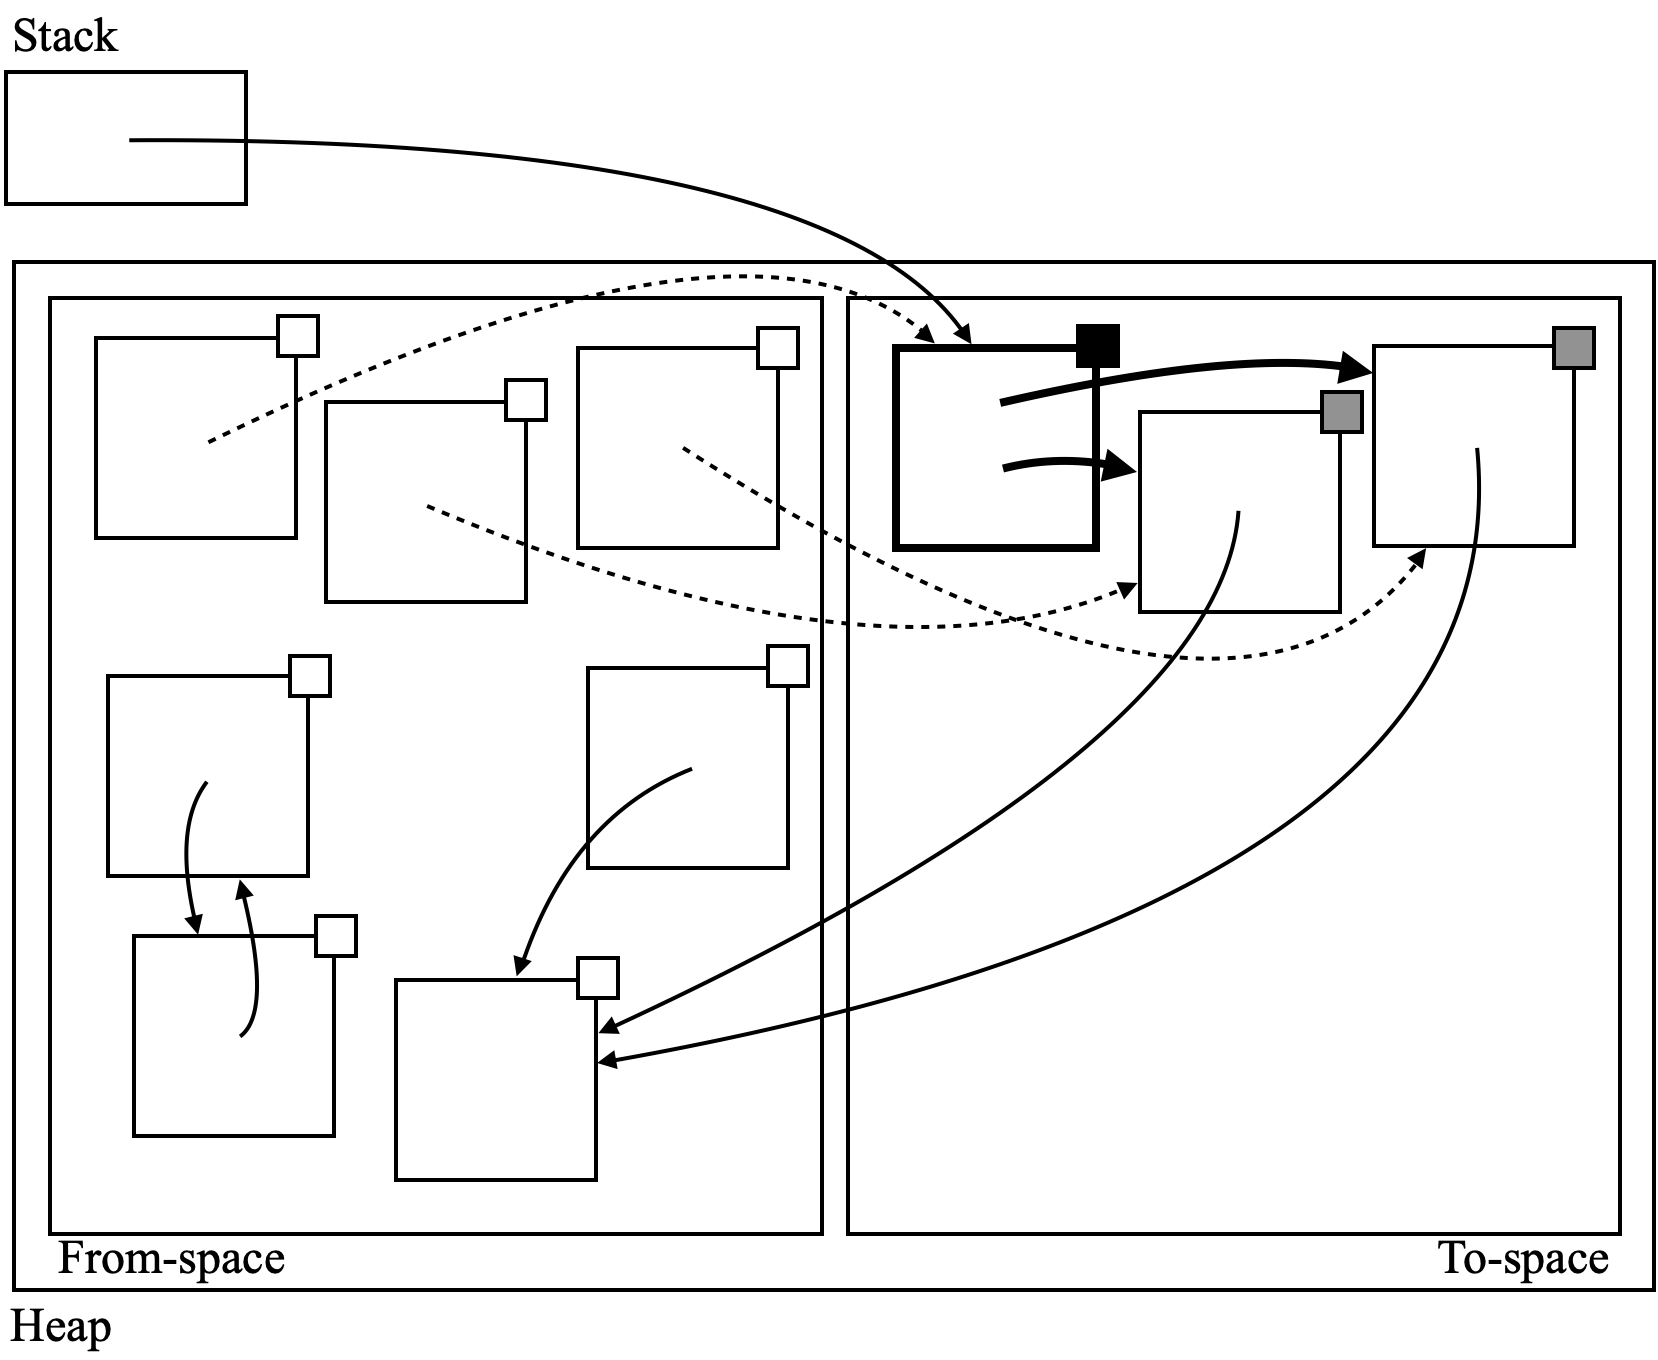
\includegraphics[height=20em]{copying3}
\end{center}

This repeats until there is no \uscn object.

\begin{center}
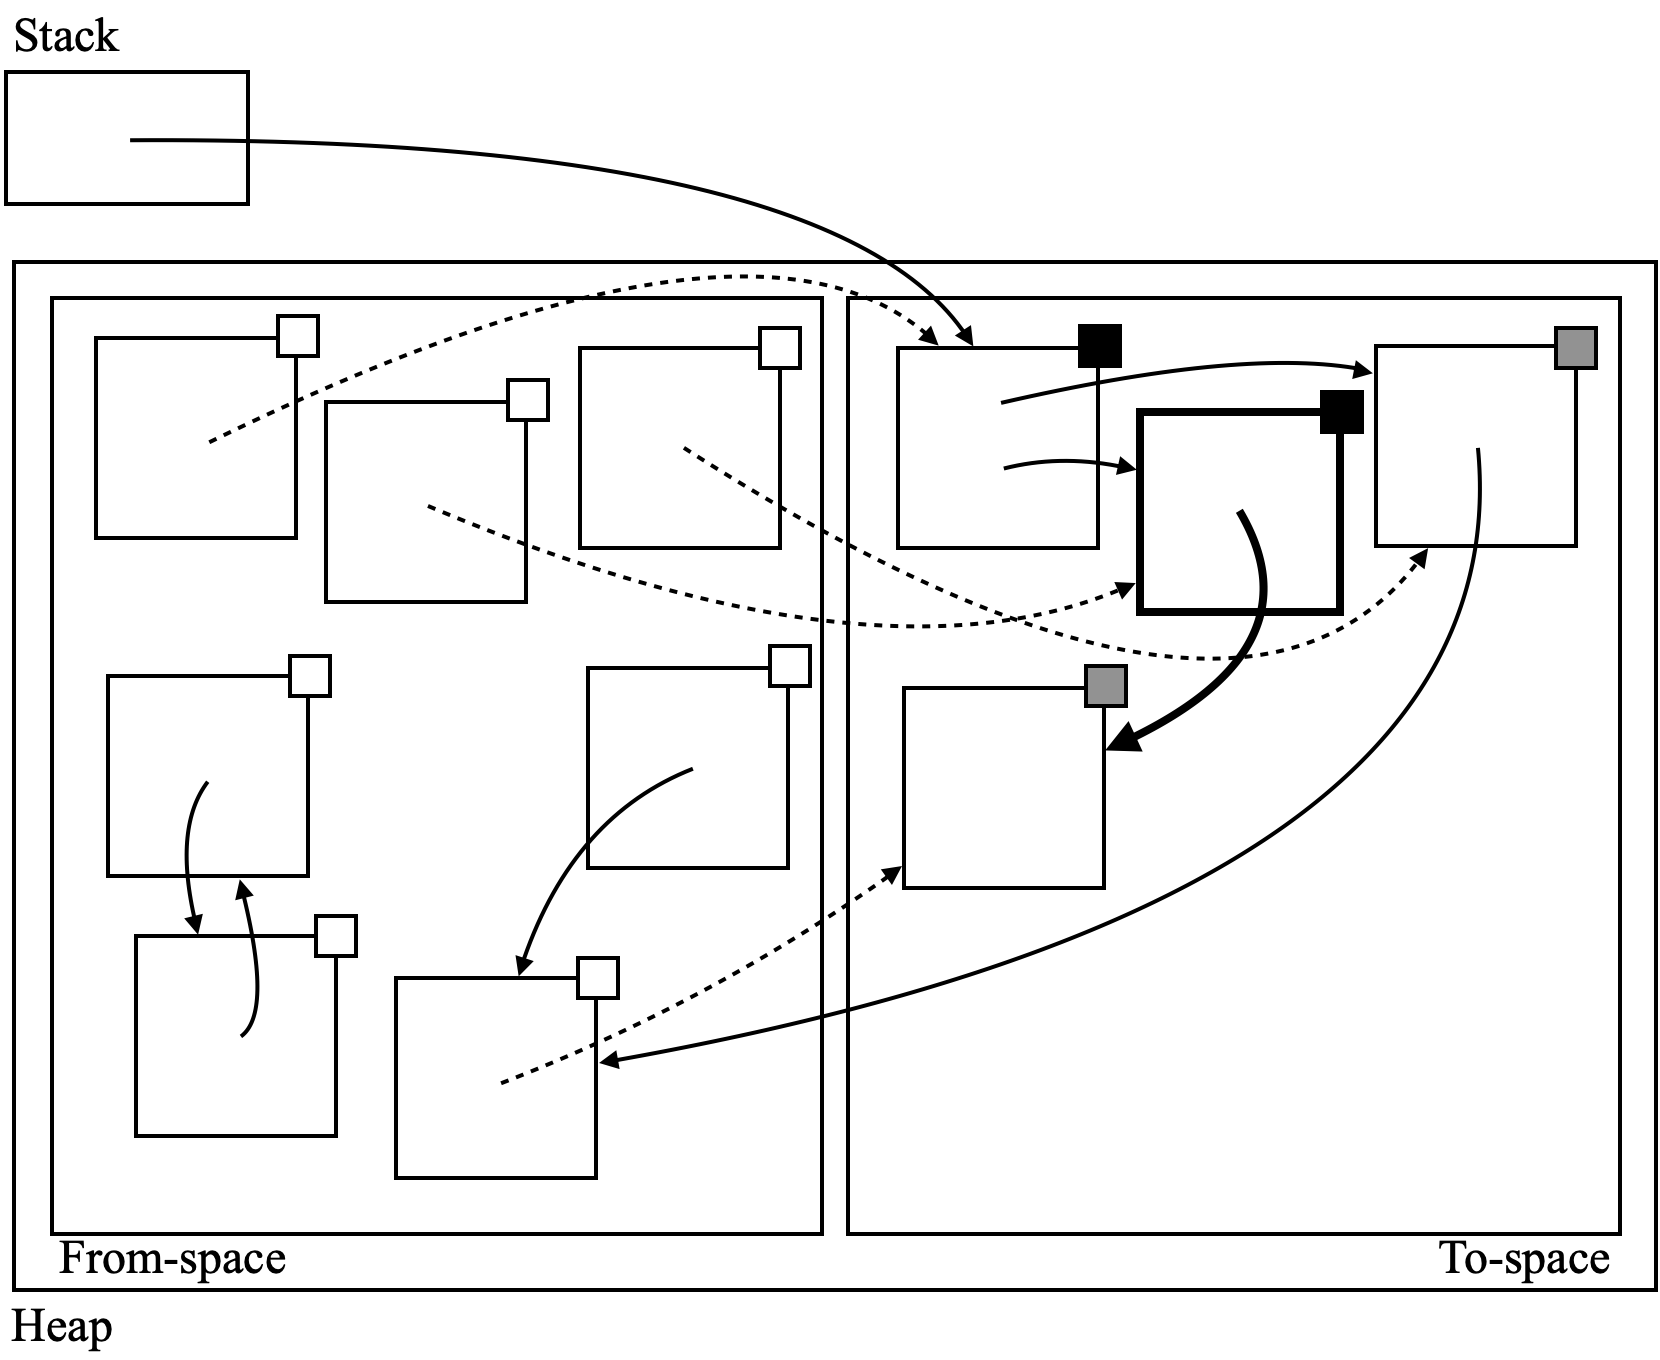
\includegraphics[height=20em]{copying4}
\end{center}

When an object pointed by a pointer has been copied to the to-space already, the
memory manager does not copy the object again and simply updates the pointer by
checking the forwarding pointer.

\begin{center}
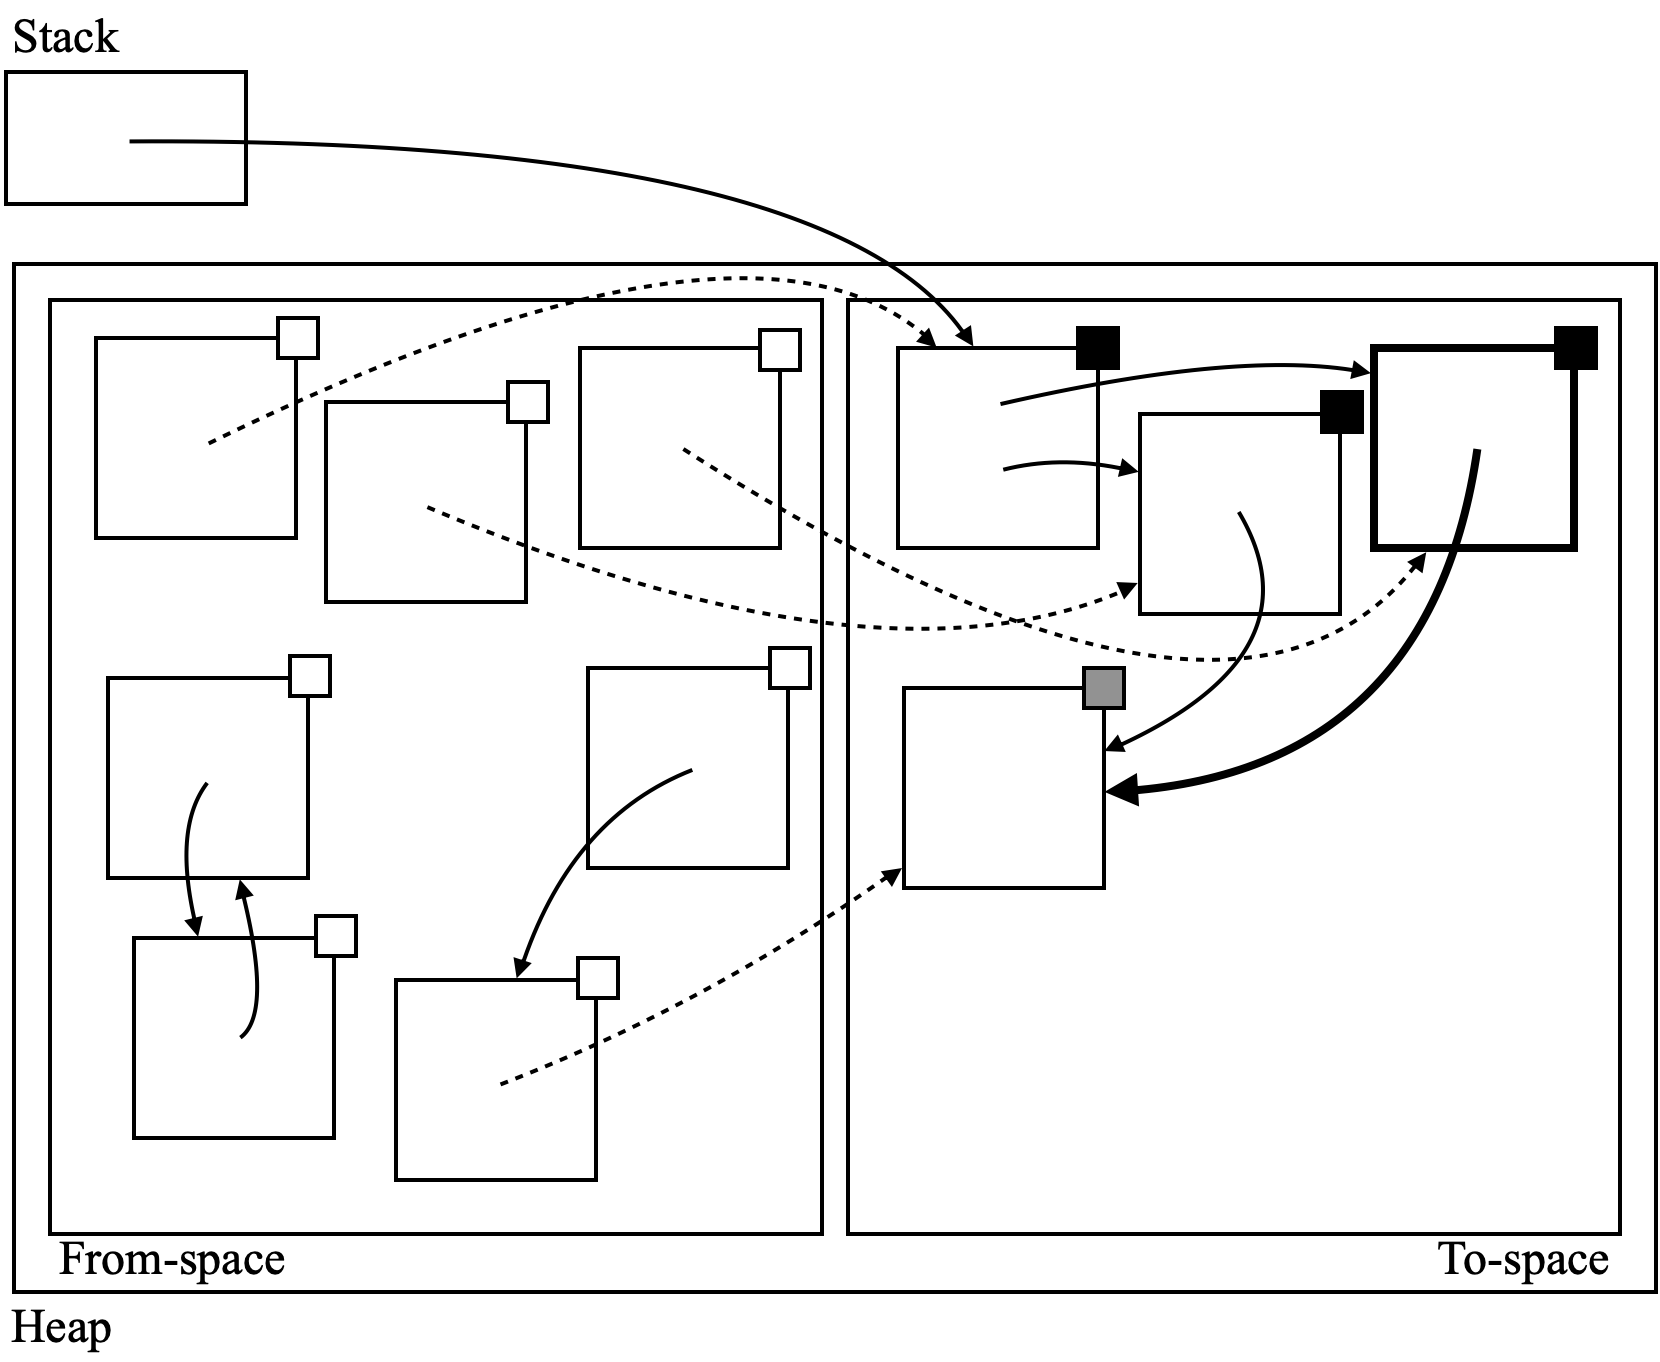
\includegraphics[height=20em]{copying5}

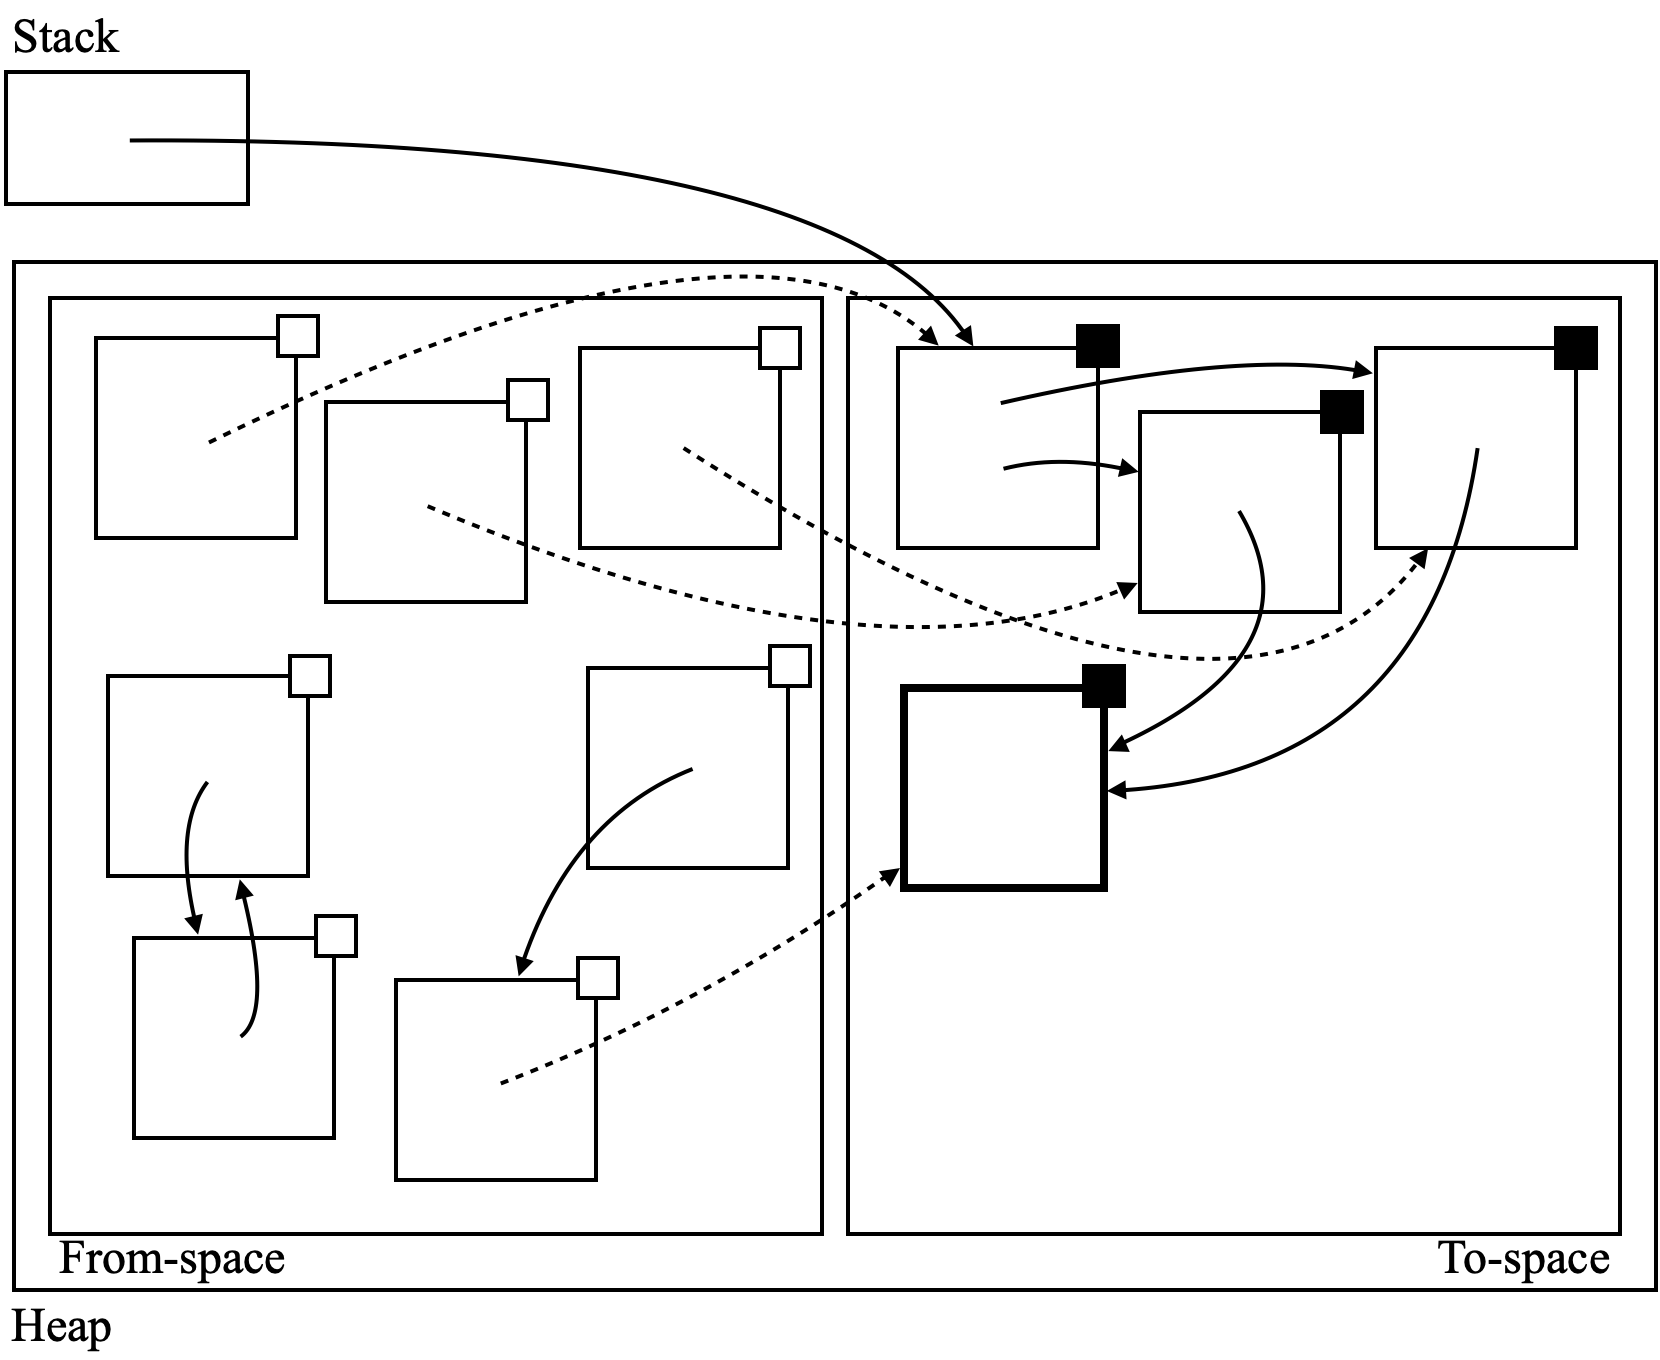
\includegraphics[height=20em]{copying6}
\end{center}

If there is no \uscn object, GC ends. The from-space and the to-space are
swapped. Now, all the allocations happen in the new from-space, and the new
to-space is considered empty.

\begin{center}
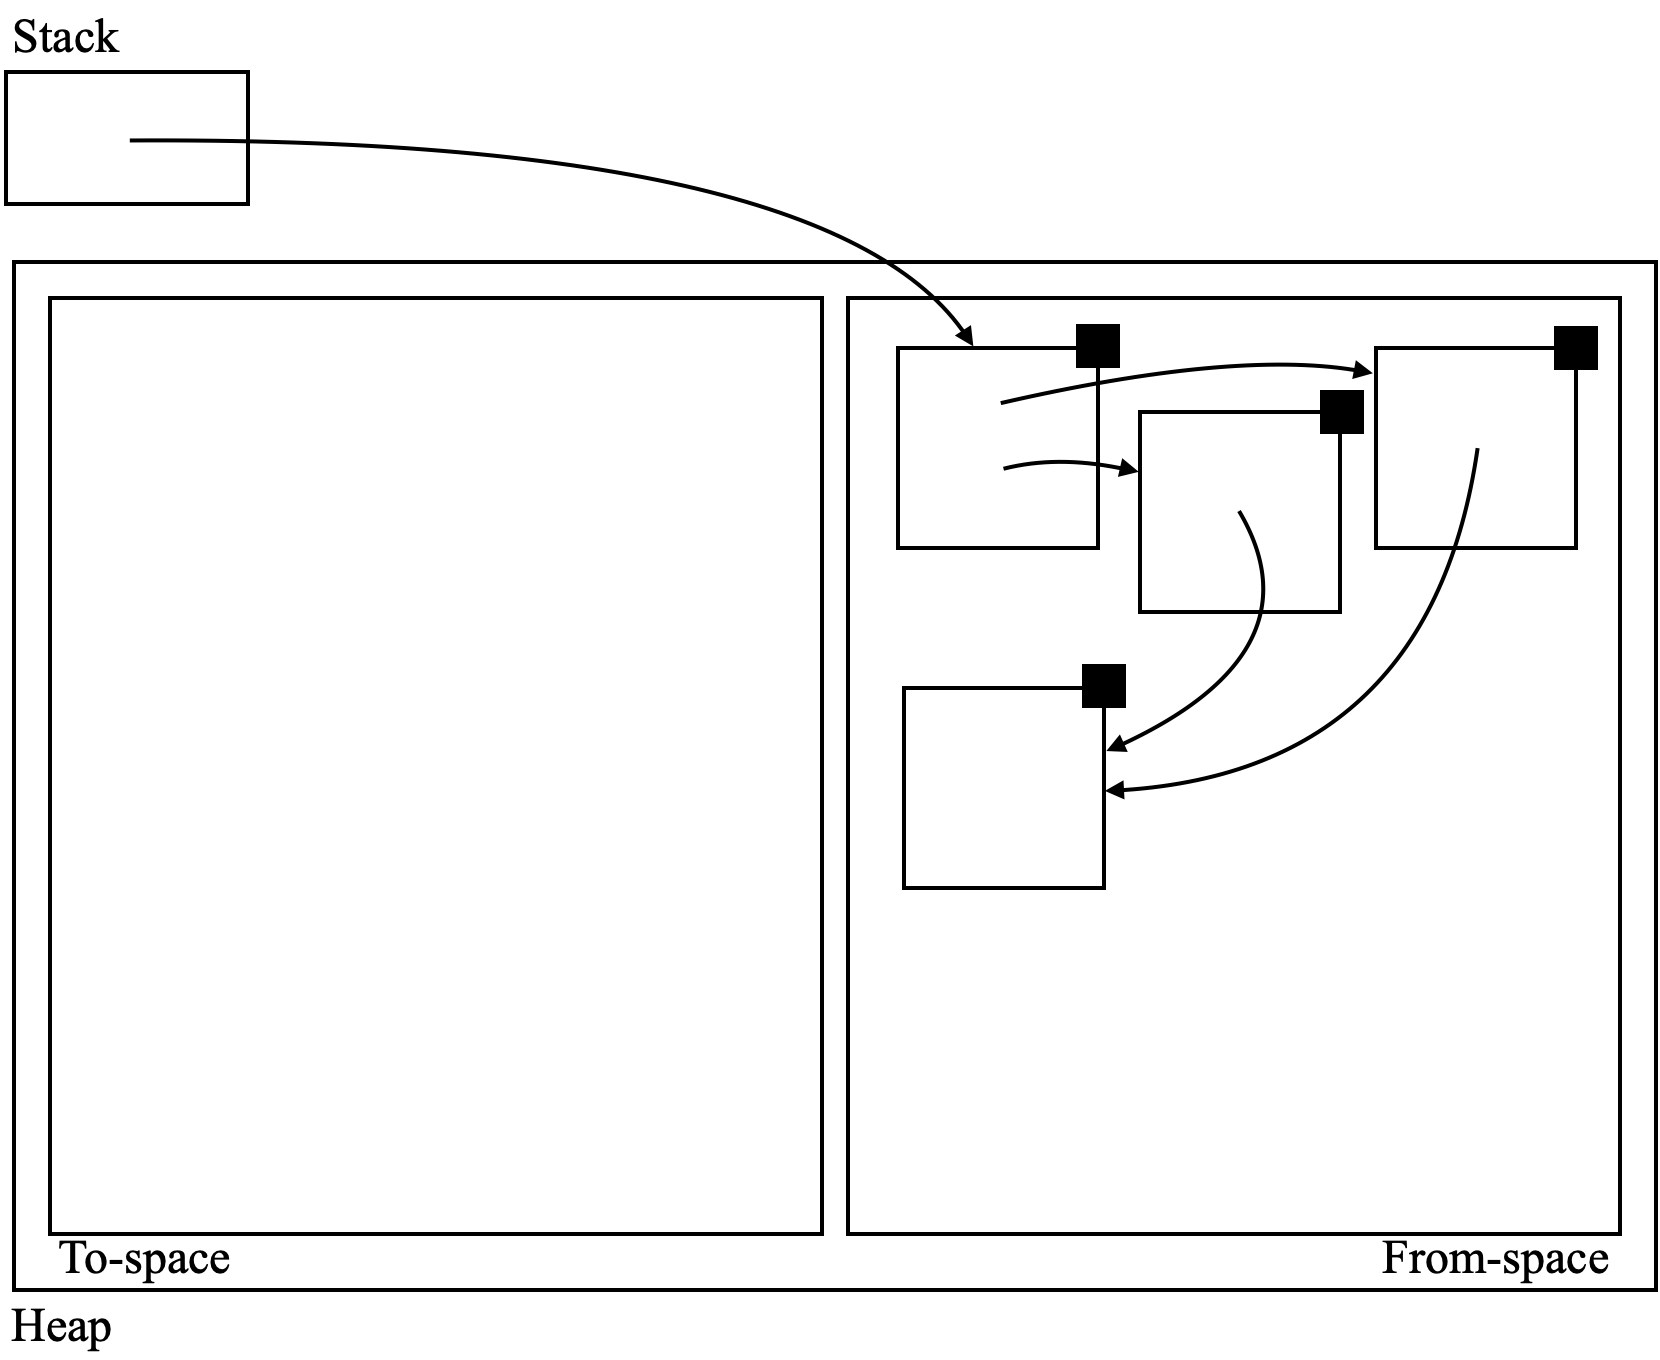
\includegraphics[height=20em]{copying7}
\end{center}

\paragraph{Cheney's Algorithm}

\newcommand{\scan}{\textsf{scan}\xspace}
\newcommand{\free}{\textsf{free}\xspace}

\textit{Cheney's algorithm}\index{Cheney's algorithm} is an efficient
implementation of copying GC. It maintains two pointers to the to-space during
GC:

\begin{itemize}
  \item \free: a pointer to the beginning of the free space of the to-space
  \item \scan: a pointer to the first \uscn object in the to-space
\end{itemize}

We use the same example as before to illustrate how Cheney's algorithm works.

\begin{center}
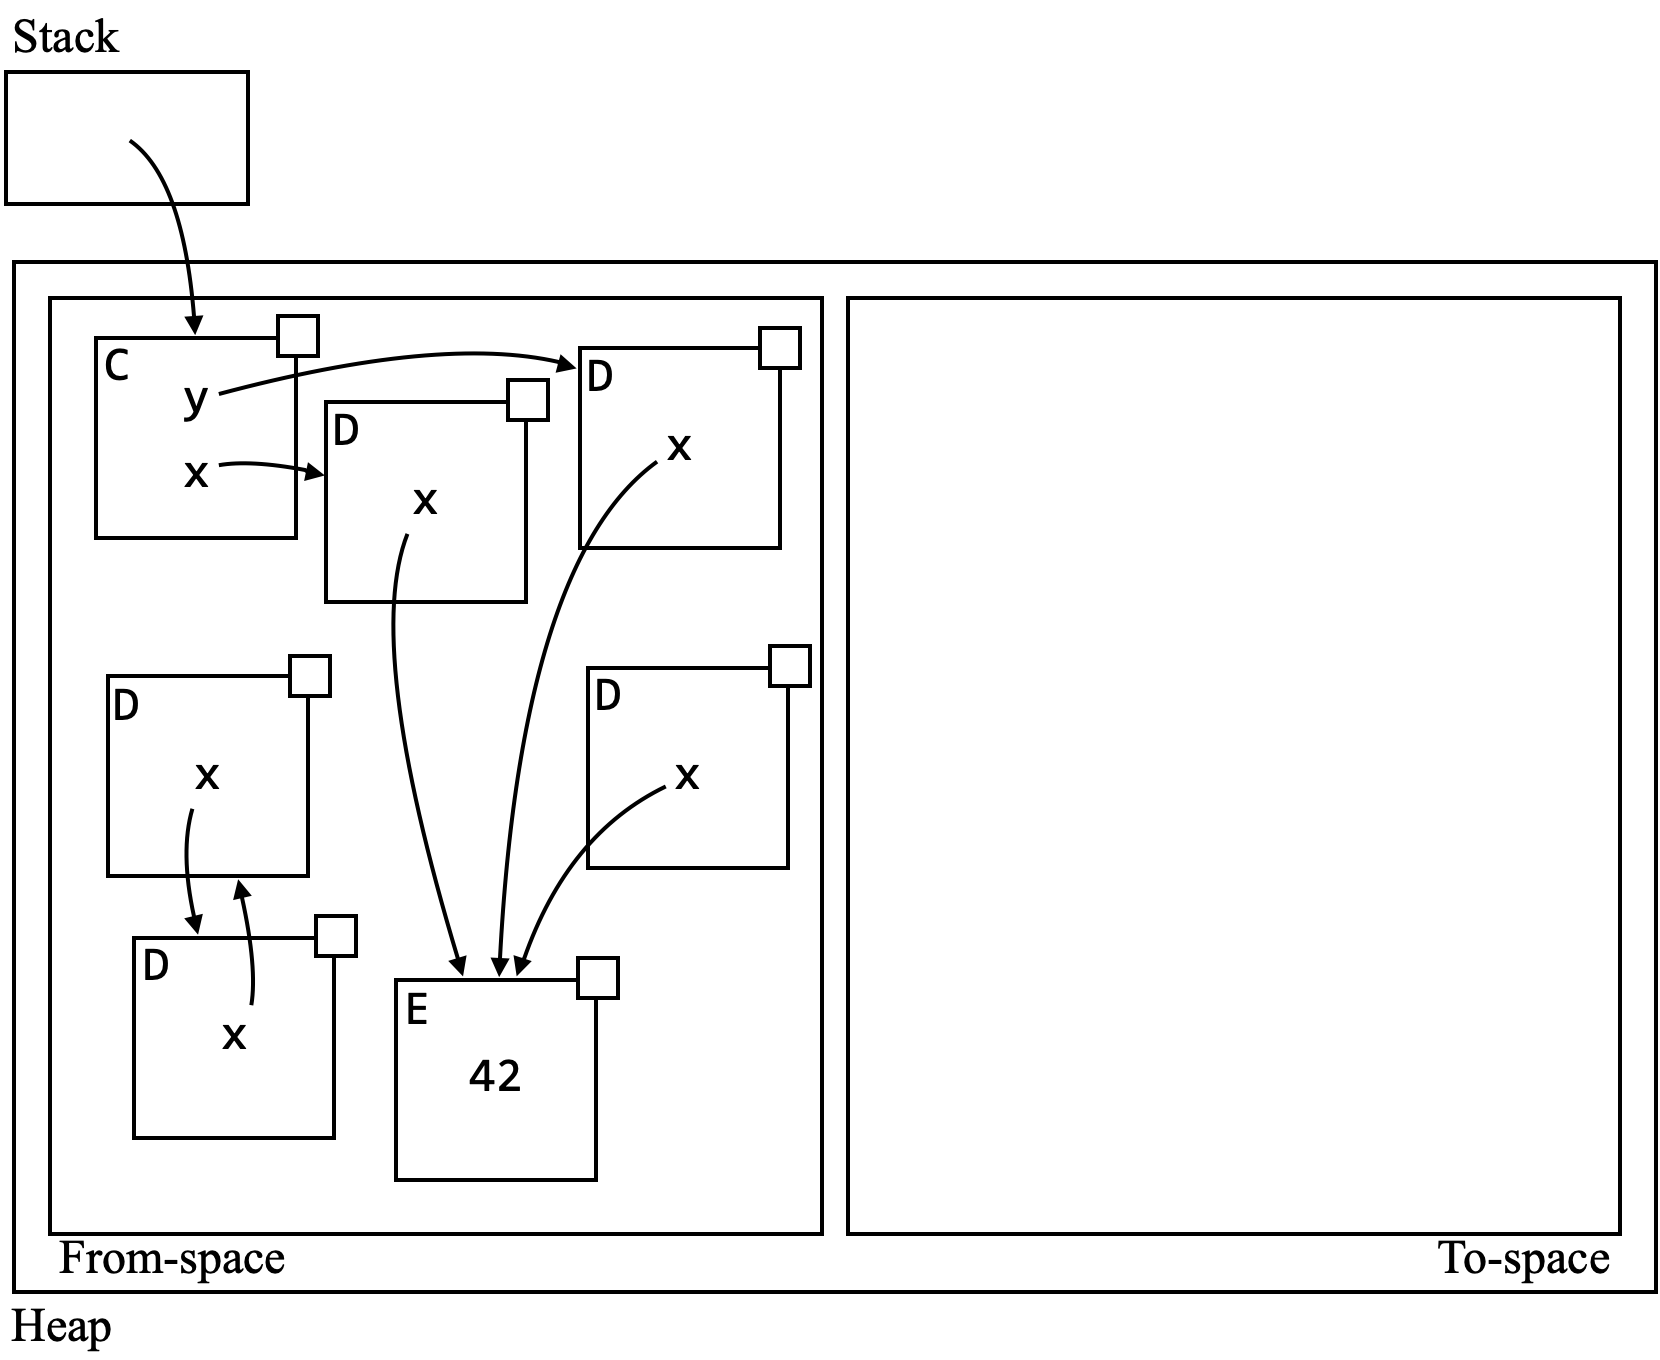
\includegraphics[height=20em]{copying-class}
\end{center}

Note that \code{C}, \code{D}, and \code{E} are classes defined as below.

\begin{verbatim}
case class C(x: AnyRef, y: AnyRef)
case class D(x: AnyRef)
case class E(x: Int)
\end{verbatim}

\code{AnyRef} is the type of any objects.

Suppose that each object in the memory has a type tag, which is the name of the
class to which the object belongs. This allows the memory manager to distinguish
pointers from integers by checking the types of fields. For example,
\code{E(42)} is represented as
$\begin{array}{|c|c|}\hline\code{E}&\code{42}\\\hline\end{array}$, and the
memory manager knows that \code{42} is an integer, not a pointer, because the
type of the field \code{x} is \code{Int}.

Now, assume that the heap is 32B-large, and each type tag, integer, and
address occupies only one byte. Then, the memory before GC is as follows:

{\small
\begin{tabular}{|@{}c@{}|@{}c@{}|@{}c@{}|@{}c@{}|@{}c@{}|@{}c@{}|@{}c@{}|@{}c@{}|@{}c@{}|@{}c@{}|@{}c@{}|@{}c@{}|@{}c@{}|@{}c@{}|@{}c@{}|@{}c@{}|@{}}
  \multicolumn{16}{@{}l}{Stack} \\
  \cline{1-1} \code{0x02} \\
  \cline{1-1}
  \multicolumn{16}{@{}l}{From-space} \\
  \hline
  \code{0x00} & \code{0x01} & \code{0x02} & \code{0x03} & \code{0x04} &
  \code{0x05} & \code{0x06} & \code{0x07} & \code{0x08} & \code{0x09} &
  \code{0x0a} & \code{0x0b} & \code{0x0c} & \code{0x0d} & \code{0x0e} &
  \code{0x0f} \\
  \hline
  \code{D} & \code{0x07} & \code{C} & \code{0x05} & \code{0x0d} &
  \code{D} & \code{0x0b} & \code{D} & \code{0x00} & \code{D} &
  \code{0x0b} & \code{E} & \code{42} & \code{D} & \code{0x0b} & \\
  \hline \multicolumn{16}{@{}l}{To-space} \\
  \hline
  \code{0x10} & \code{0x11} & \code{0x12} & \code{0x13} & \code{0x14} &
  \code{0x15} & \code{0x16} & \code{0x17} & \code{0x18} & \code{0x19} &
  \code{0x1a} & \code{0x1b} & \code{0x1c} & \code{0x1d} & \code{0x1e} &
  \code{0x1f} \\
  \hline
  &&&&&&&&&&&&&&& \\
  \hline
  \hline
  \scan &&&&&&&&&&&&&&& \\
  \free &&&&&&&&&&&&&&& \\
  \hline
\end{tabular}
}

The first row of each space shows the address of each slot, and the second row
shows the content of the space. The last row shows the locations of \scan and
\free.  In the beginning, both \scan and \free point to the beginning of the
to-space because the to-space is empty.

As the first step, the only object directly pointed by the stack is copied.

{\small
\begin{tabular}{|@{}c@{}|@{}c@{}|@{}c@{}|@{}c@{}|@{}c@{}|@{}c@{}|@{}c@{}|@{}c@{}|@{}c@{}|@{}c@{}|@{}c@{}|@{}c@{}|@{}c@{}|@{}c@{}|@{}c@{}|@{}c@{}|@{}}
  \multicolumn{16}{@{}l}{Stack} \\
  \cline{1-1} \inred\code{0x10} \\
  \cline{1-1}
  \multicolumn{16}{@{}l}{From-space} \\
  \hline
  \code{0x00} & \code{0x01} & \code{0x02} & \code{0x03} & \code{0x04} &
  \code{0x05} & \code{0x06} & \code{0x07} & \code{0x08} & \code{0x09} &
  \code{0x0a} & \code{0x0b} & \code{0x0c} & \code{0x0d} & \code{0x0e} &
  \code{0x0f} \\
  \hline
  \code{D} & \code{0x07} & \inred\code{F} & \inred\code{0x10} & \code{0x0d} &
  \code{D} & \code{0x0b} & \code{D} & \code{0x00} & \code{D} &
  \code{0x0b} & \code{E} & \code{42} & \code{D} & \code{0x0b} & \\
  \hline \multicolumn{16}{@{}l}{To-space} \\
  \hline
  \code{0x10} & \code{0x11} & \code{0x12} & \code{0x13} & \code{0x14} &
  \code{0x15} & \code{0x16} & \code{0x17} & \code{0x18} & \code{0x19} &
  \code{0x1a} & \code{0x1b} & \code{0x1c} & \code{0x1d} & \code{0x1e} &
  \code{0x1f} \\
  \hline
  \inred\code{C} & \inred\code{0x05} & \inred\code{0x0d} &&&&&&&&&&&&& \\
  \hline
  \hline
  \scan &&&&&&&&&&&&&&& \\
  &&& \inred\free &&&&&&&&&&&& \\
  \hline
\end{tabular}
}

\code{F} is the type tag of an object that has been copied already. An object with
the type tag \code{F} has a forwarding pointer. The to-space now has an object,
so the \code{free} pointer advances by the size of the object. On the other
hand, the object has not been scanned yet, so the \code{scan} pointer stays
still. It shows that the objects between \code{scan} and \code{free} are \uscn
objects.

As the next step, the object pointed by \code{scan} is scanned. All the objects
pointed by the object being scanned are copied.

{\small
\begin{tabular}{|@{}c@{}|@{}c@{}|@{}c@{}|@{}c@{}|@{}c@{}|@{}c@{}|@{}c@{}|@{}c@{}|@{}c@{}|@{}c@{}|@{}c@{}|@{}c@{}|@{}c@{}|@{}c@{}|@{}c@{}|@{}c@{}|@{}}
  \multicolumn{16}{@{}l}{Stack} \\
  \cline{1-1} \code{0x10} \\
  \cline{1-1}
  \multicolumn{16}{@{}l}{From-space} \\
  \hline
  \code{0x00} & \code{0x01} & \code{0x02} & \code{0x03} & \code{0x04} &
  \code{0x05} & \code{0x06} & \code{0x07} & \code{0x08} & \code{0x09} &
  \code{0x0a} & \code{0x0b} & \code{0x0c} & \code{0x0d} & \code{0x0e} &
  \code{0x0f} \\
  \hline
  \code{D} & \code{0x07} & \code{F} & \code{0x10} & \code{0x0d} &
  \inred\code{F} & \inred\code{0x13} & \code{D} & \code{0x00} & \code{D} &
  \code{0x0b} & \code{E} & \code{42} & \inred\code{F} & \inred\code{0x15} & \\
  \hline \multicolumn{16}{@{}l}{To-space} \\
  \hline
  \code{0x10} & \code{0x11} & \code{0x12} & \code{0x13} & \code{0x14} &
  \code{0x15} & \code{0x16} & \code{0x17} & \code{0x18} & \code{0x19} &
  \code{0x1a} & \code{0x1b} & \code{0x1c} & \code{0x1d} & \code{0x1e} &
  \code{0x1f} \\
  \hline
  \code{C} & \inred\code{0x13} & \inred\code{0x15} & \inred\code{D} & \inred\code{0x0b} & \inred\code{D} &
  \inred\code{0x0b} &&&&&&&&& \\
  \hline
  \hline
  &&& \inred\scan &&&&&&&&&&&& \\
  &&&&&&& \inred\free &&&&&&&& \\
  \hline
\end{tabular}
}

The \code{free} pointer advances again by the sum of the sizes of all the copied
objects. In addition, the \code{scan} pointer also advances to the next object
in the to-space because the object previously pointed by \code{scan} has been
scanned. Note that when the \code{scan} pointer advances, the old addresses
\code{0x05} and \code{0x0d} are updated to new addresses
\code{0x13} and \code{0x15}, respectively.
This shows that the objects before \code{scan} are \scn objects.

This repeats until \code{scan} catchs up with \code{free}, i.e., there is no
\uscn object.

{\small
\begin{tabular}{|@{}c@{}|@{}c@{}|@{}c@{}|@{}c@{}|@{}c@{}|@{}c@{}|@{}c@{}|@{}c@{}|@{}c@{}|@{}c@{}|@{}c@{}|@{}c@{}|@{}c@{}|@{}c@{}|@{}c@{}|@{}c@{}|@{}}
  \multicolumn{16}{@{}l}{Stack} \\
  \cline{1-1} \code{0x10} \\
  \cline{1-1}
  \multicolumn{16}{@{}l}{From-space} \\
  \hline
  \code{0x00} & \code{0x01} & \code{0x02} & \code{0x03} & \code{0x04} &
  \code{0x05} & \code{0x06} & \code{0x07} & \code{0x08} & \code{0x09} &
  \code{0x0a} & \code{0x0b} & \code{0x0c} & \code{0x0d} & \code{0x0e} &
  \code{0x0f} \\
  \hline
  \code{D} & \code{0x07} & \code{F} & \code{0x10} & \code{0x0d} &
  \code{F} & \code{0x13} & \code{D} & \code{0x00} & \code{D} &
  \code{0x0b} & \inred\code{F} & \inred\code{0x17} & \code{F} & \code{0x15} & \\
  \hline \multicolumn{16}{@{}l}{To-space} \\
  \hline
  \code{0x10} & \code{0x11} & \code{0x12} & \code{0x13} & \code{0x14} &
  \code{0x15} & \code{0x16} & \code{0x17} & \code{0x18} & \code{0x19} &
  \code{0x1a} & \code{0x1b} & \code{0x1c} & \code{0x1d} & \code{0x1e} &
  \code{0x1f} \\
  \hline
  \code{C} & \code{0x13} & \code{0x15} & \code{D} & \inred\code{0x17} & \code{D} &
  \code{0x0b} & \inred\code{E} & \inred\code{42} &&&&&&& \\
  \hline
  \hline
  &&&&& \inred\scan &&&&&&&&&& \\
  &&&&&&&&& \inred\free &&&&&& \\
  \hline
\end{tabular}
}

{\small
\begin{tabular}{|@{}c@{}|@{}c@{}|@{}c@{}|@{}c@{}|@{}c@{}|@{}c@{}|@{}c@{}|@{}c@{}|@{}c@{}|@{}c@{}|@{}c@{}|@{}c@{}|@{}c@{}|@{}c@{}|@{}c@{}|@{}c@{}|@{}}
  \multicolumn{16}{@{}l}{Stack} \\
  \cline{1-1} \code{0x10} \\
  \cline{1-1}
  \multicolumn{16}{@{}l}{From-space} \\
  \hline
  \code{0x00} & \code{0x01} & \code{0x02} & \code{0x03} & \code{0x04} &
  \code{0x05} & \code{0x06} & \code{0x07} & \code{0x08} & \code{0x09} &
  \code{0x0a} & \code{0x0b} & \code{0x0c} & \code{0x0d} & \code{0x0e} &
  \code{0x0f} \\
  \hline
  \code{D} & \code{0x07} & \code{F} & \code{0x10} & \code{0x0d} &
  \code{F} & \code{0x13} & \code{D} & \code{0x00} & \code{D} &
  \code{0x0b} & \code{F} & \code{0x17} & \code{F} & \code{0x15} & \\
  \hline \multicolumn{16}{@{}l}{To-space} \\
  \hline
  \code{0x10} & \code{0x11} & \code{0x12} & \code{0x13} & \code{0x14} &
  \code{0x15} & \code{0x16} & \code{0x17} & \code{0x18} & \code{0x19} &
  \code{0x1a} & \code{0x1b} & \code{0x1c} & \code{0x1d} & \code{0x1e} &
  \code{0x1f} \\
  \hline
  \code{C} & \code{0x13} & \code{0x15} & \code{D} & \code{0x17} & \code{D} &
  \inred\code{0x17} & \code{E} & \code{42} &&&&&&& \\
  \hline
  \hline
  &&&&&&& \inred\scan &&&&&&&& \\
  &&&&&&&&& \free &&&&&& \\
  \hline
\end{tabular}
}

{\small
\begin{tabular}{|@{}c@{}|@{}c@{}|@{}c@{}|@{}c@{}|@{}c@{}|@{}c@{}|@{}c@{}|@{}c@{}|@{}c@{}|@{}c@{}|@{}c@{}|@{}c@{}|@{}c@{}|@{}c@{}|@{}c@{}|@{}c@{}|@{}}
  \multicolumn{16}{@{}l}{Stack} \\
  \cline{1-1} \code{0x10} \\
  \cline{1-1}
  \multicolumn{16}{@{}l}{From-space} \\
  \hline
  \code{0x00} & \code{0x01} & \code{0x02} & \code{0x03} & \code{0x04} &
  \code{0x05} & \code{0x06} & \code{0x07} & \code{0x08} & \code{0x09} &
  \code{0x0a} & \code{0x0b} & \code{0x0c} & \code{0x0d} & \code{0x0e} &
  \code{0x0f} \\
  \hline
  \code{D} & \code{0x07} & \code{F} & \code{0x10} & \code{0x0d} &
  \code{F} & \code{0x13} & \code{D} & \code{0x00} & \code{D} &
  \code{0x0b} & \code{F} & \code{0x17} & \code{F} & \code{0x15} & \\
  \hline \multicolumn{16}{@{}l}{To-space} \\
  \hline
  \code{0x10} & \code{0x11} & \code{0x12} & \code{0x13} & \code{0x14} &
  \code{0x15} & \code{0x16} & \code{0x17} & \code{0x18} & \code{0x19} &
  \code{0x1a} & \code{0x1b} & \code{0x1c} & \code{0x1d} & \code{0x1e} &
  \code{0x1f} \\
  \hline
  \code{C} & \code{0x13} & \code{0x15} & \code{D} & \code{0x17} & \code{D} &
  \code{0x17} & \code{E} & \code{42} &&&&&&& \\
  \hline
  \hline
  &&&&&&&&& \inred\scan &&&&&& \\
  &&&&&&&&& \free &&&&&& \\
  \hline
\end{tabular}
}

\subsection{Pros}

The copying GC has the following strengths:

\begin{itemize}
  \item It can handle cyclic structures.
  \item Allocations are extremely fast.
  \item It does not suffer from external fragmentation.
\end{itemize}

Like mark-and-sweep GC, copying GC can handle cyclic structures.

\paragraph{Fast Allocation}

Copying GC does not require free lists. The \code{free} pointer used by Cheney's
algorithm is enough. Objects are contiguously allocated at the beginning of the
from-space, and GC copies reachable objects to the beginning of the to-space
instead of selectively deallocating unreachable objects. For this reason, the
free space of the heap is always a single continuous block of memory, and every
new object can be allocated at the address to which \code{free} points. It
allows constant-time allocation. It is much faster than reference counting and
mark-and-sweep GC, which need to traverse free lists.

\paragraph{No External Fragmentation}

Since the free space is always a single memory block, there is no external
fragmentation. It allows efficient use of the heap; if there is enough space,
objects can be always allocated. In addition, it guarantees good locality;
consecutive allocations always result in contiguous objects on the heap.

\subsection{Cons}

The copying GC has the following weaknesses:

\begin{itemize}
  \item Execution stops during GC.
  \item Only a half of the heap can store objects.
  \item Copying is expensive.
\end{itemize}

Like mark-and-sweep GC, programs pause for a while when GC is triggered.

\paragraph{Small Free Space}

Since copying GC divides the heap into two pieces, only a half of the heap is
available for allocating objects. It leads to more frequent GC, which pauses
execution.

\paragraph{Cost of Copying}

Unlike reference counting and mark-and-sweep GC, copying GC copies reachable
objects every time GC is triggered. If the heap has a large ammount of reachable
objects, copying will take a long time and increase the duration of the pause.

\section{Exercises}

\begin{enumerate}
\item
 When a program runs out of memory,
    \ansbox{a} finds inaccessible inaccessible objects and deallocates
    them to make free space. There are three well-known strategies to
    implement \ansbox{a}.
\begin{itemize}
\item \ansbox{b} divides memory into two regions: to-space and
  from-space. New allocations happen in to-space. When to-space
  becomes full, to-space and from-space are swapped first, and then
  live objects are copied from from-space to to-space.
\item \ansbox{c} marks all the reachable objects from root
  objects. After the traversal, every un- marked object is freed.
\item \ansbox{d} tracks how many objects point to a certain
  object. When an object is not referred by anything, the object is freed.
\end{itemize}

Fill from (a) to (d) with the following terms.

\begin{center}
\begin{tabular}{|c|}
  \hline
  reference counting \qquad mark and sweep \\[6pt]
  garbage collection \qquad copying \\ \hline
\end{tabular}
\end{center}

\item
 The Swift programming language uses the reference counting garbage collection algorithm.

\begin{enumerate}
  \item
What is the correct order?

\begin{enumerate}
\item When a count is decremented to 0, decrement counts for other records referenced by the record, then free it
\item When replacing a pointer to a record, decrement its count
\item Attatch a count to every record, starting at 0
\item When installing a pointer to a record, increment its count
\end{enumerate}

  \item Provide an example that shows why the order matters.

\end{enumerate}

\item Suppose a garbage-collected interepreter uses the following five kinds of records:

  \begin{itemize}
  \item Tag \textbf{1}: a record containing two pointers
  \item Tag \textbf{2}: a record containing one pointer and one integer
  \item Tag \textbf{3}: a record containing one integer
  \item Tag \textbf{4}: a record containing one integer and one pointer
  \item Tag \textbf{99}: forwarding pointer (to to-space)
  \end{itemize}

 The interpreter has one register, which always contains a pointer,
 and a memory pool of size 26. The allocator/collector is a two-space
 copying collector, so each space is of size 13. Records are allocated
 consecutively in to-space, starting from the first memory location,
 0.

 The following is a snapshot of memory just before a collection where
 all memory has been allocated:

 \begin{itemize}
 \item Register: 8
 \item From space: 1 3 8 3 0 4 7 3 2 0 8 3 42
 \end{itemize}

What are the values in the register, the from-space, and the to-space after collection?
Assume that unallocated memory in to-space contains 0.

 \begin{itemize}
 \item Register:

 \item From space:

 \item To space:
 \end{itemize}

\item
Suppose a garbage-collected interepreter uses the following five kinds of records:

  \begin{itemize}
  \item Tag \textbf{1}: a record containing one integer
  \item Tag \textbf{2}: a record containing one integer and one pointer
  \item Tag \textbf{3}: a record containing one pointer and one integer
  \item Tag \textbf{4}: a record containing two pointers
  \item Tag \textbf{99}: forwarding pointer (to to-space)
  \end{itemize}

 The interpreter has one register, which always contains a pointer,
 and a memory pool of size 26. The allocator/collector is a two-space
 copying collector, so each space is of size 13. Records are allocated
 consecutively in to-space, starting from the first memory location,
 0.

 The following is a snapshot of memory just before a collection where
 all memory has been allocated:

 \begin{itemize}
 \item Register: 8
 \item From space:
 \begin{tabular}{|c|c|c|c|c|c|c|c|c|c|c|c|@{\hskip0pt}c@{\hskip0pt}|}
  \hline
  4&3&8&1&5&2&7&0&3&0&2&1&42\\
  \hline \multicolumn{1}{c}{}\\[-16pt]
  \multicolumn{1}{c}{\tiny 0}&
  \multicolumn{1}{c}{\tiny 1}&
  \multicolumn{1}{c}{\tiny 2}&
  \multicolumn{1}{c}{\tiny 3}&
  \multicolumn{1}{c}{\tiny 4}&
  \multicolumn{1}{c}{\tiny 5}&
  \multicolumn{1}{c}{\tiny 6}&
  \multicolumn{1}{c}{\tiny 7}&
  \multicolumn{1}{c}{\tiny 8}&
  \multicolumn{1}{c}{\tiny 9}&
  \multicolumn{1}{c}{\tiny 10}&
  \multicolumn{1}{c}{\tiny 11}&
  \multicolumn{1}{c}{\tiny 12}
  \\
 \end{tabular}
 \end{itemize}

What are the values in the register, the from-space, and the to-space after collection?
Assume that unallocated memory in the to-space contains 0, the from-space uses
addresses from 0 to 12, and the to-space uses addresses from 13 to 25.

 \begin{itemize}
 \item Register: \\[10pt]
 {\Huge
 \begin{tabular}{|c|}
  \hline~~~\\ \hline
 \end{tabular}
 }

 \item From space: \\[10pt]
 {\Huge
 \begin{tabular}{|c|c|c|c|c|c|c|c|c|c|c|c|c|}
  \hline~~~&~~~&~~~&~~~&~~~&~~~&~~~&~~~&~~~&~~~&~~~&~~~&~~~\\
  \hline \multicolumn{1}{c}{}\\[-46pt]
  \multicolumn{1}{c}{\tiny 0}&
  \multicolumn{1}{c}{\tiny 1}&
  \multicolumn{1}{c}{\tiny 2}&
  \multicolumn{1}{c}{\tiny 3}&
  \multicolumn{1}{c}{\tiny 4}&
  \multicolumn{1}{c}{\tiny 5}&
  \multicolumn{1}{c}{\tiny 6}&
  \multicolumn{1}{c}{\tiny 7}&
  \multicolumn{1}{c}{\tiny 8}&
  \multicolumn{1}{c}{\tiny 9}&
  \multicolumn{1}{c}{\tiny 10}&
  \multicolumn{1}{c}{\tiny 11}&
  \multicolumn{1}{c}{\tiny 12}
  \\
 \end{tabular}
 }
 \item To space: \\[10pt]
 {\Huge
 \begin{tabular}{|c|c|c|c|c|c|c|c|c|c|c|c|c|}
  \hline~~~&~~~&~~~&~~~&~~~&~~~&~~~&~~~&~~~&~~~&~~~&~~~&~~~\\
  \hline \multicolumn{1}{c}{}\\[-46pt]
  \multicolumn{1}{c}{\tiny 13}&
  \multicolumn{1}{c}{\tiny 14}&
  \multicolumn{1}{c}{\tiny 15}&
  \multicolumn{1}{c}{\tiny 16}&
  \multicolumn{1}{c}{\tiny 17}&
  \multicolumn{1}{c}{\tiny 18}&
  \multicolumn{1}{c}{\tiny 19}&
  \multicolumn{1}{c}{\tiny 20}&
  \multicolumn{1}{c}{\tiny 21}&
  \multicolumn{1}{c}{\tiny 22}&
  \multicolumn{1}{c}{\tiny 23}&
  \multicolumn{1}{c}{\tiny 24}&
  \multicolumn{1}{c}{\tiny 25}
 \end{tabular}
 }
 \end{itemize}

\item
Suppose a garbage-collected interepreter uses the following five kinds of records:

  \begin{itemize}
  \item Tag \textbf{1}: a record containing one integer
  \item Tag \textbf{2}: a record containing one integer and one pointer
  \item Tag \textbf{3}: a record containing one pointer and one integer
  \item Tag \textbf{4}: a record containing two pointers
  \item Tag \textbf{99}: forwarding pointer (to to-space)
  \end{itemize}

 The interpreter has one register, which always contains a pointer,
 and a memory pool of size 26. The allocator/collector is a two-space
 copying collector, so each space is of size 13. Records are allocated
 consecutively in to-space, starting from the first memory location,
 0.

 The following is the snapshot of the memory just before garbage collection,
 where all the memory has been allocated:

 \begin{itemize}
 \item Register: 8
 \item From space:
 \begin{tabular}{|c|c|c|c|c|c|c|c|c|c|c|c|@{\hskip0pt}c@{\hskip0pt}|}
  \hline
  4&3&8&1&9&2&8&0&3&0&0&1&6\\
  \hline \multicolumn{1}{c}{}\\[-16pt]
  \multicolumn{1}{c}{\tiny 0}&
  \multicolumn{1}{c}{\tiny 1}&
  \multicolumn{1}{c}{\tiny 2}&
  \multicolumn{1}{c}{\tiny 3}&
  \multicolumn{1}{c}{\tiny 4}&
  \multicolumn{1}{c}{\tiny 5}&
  \multicolumn{1}{c}{\tiny 6}&
  \multicolumn{1}{c}{\tiny 7}&
  \multicolumn{1}{c}{\tiny 8}&
  \multicolumn{1}{c}{\tiny 9}&
  \multicolumn{1}{c}{\tiny 10}&
  \multicolumn{1}{c}{\tiny 11}&
  \multicolumn{1}{c}{\tiny 12}
  \\
 \end{tabular}
 \item To space:
 \begin{tabular}{|c|c|c|c|c|c|c|c|c|c|c|c|@{\hskip0pt}c@{\hskip0pt}|}
  \hline
  0&0&0&0&0&0&0&0&0&0&0&0&0\\
  \hline \multicolumn{1}{c}{}\\[-16pt]
  \multicolumn{1}{c}{\tiny 13}&
  \multicolumn{1}{c}{\tiny 14}&
  \multicolumn{1}{c}{\tiny 15}&
  \multicolumn{1}{c}{\tiny 16}&
  \multicolumn{1}{c}{\tiny 17}&
  \multicolumn{1}{c}{\tiny 18}&
  \multicolumn{1}{c}{\tiny 19}&
  \multicolumn{1}{c}{\tiny 20}&
  \multicolumn{1}{c}{\tiny 21}&
  \multicolumn{1}{c}{\tiny 22}&
  \multicolumn{1}{c}{\tiny 23}&
  \multicolumn{1}{c}{\tiny 24}&
  \multicolumn{1}{c}{\tiny 25}
  \\
 \end{tabular}
 \end{itemize}

What are the values in the register, the from-space, and the to-space after
garbage collection? Draw your answer just like the above figure.

\item
Suppose a garbage-collected interepreter uses the following five kinds of records:

  \begin{itemize}
  \item Tag \textbf{1}: a record containing one integer
  \item Tag \textbf{2}: a record containing one integer and one pointer
  \item Tag \textbf{3}: a record containing one pointer and one integer
  \item Tag \textbf{4}: a record containing two pointers
  \item Tag \textbf{99}: forwarding pointer (to to-space)
  \end{itemize}

 The interpreter has one register, which always contains a pointer,
 and a memory pool of size 26. The allocator/collector is a two-space
 copying collector, so each space is of size 13. Records are allocated
 consecutively in to-space, starting from the first memory location,
 0.

 The following is the snapshot of the memory just before garbage collection,
 where all the memory has been allocated:

 \begin{itemize}
 \item Register: 10
 \item From space:
 \begin{tabular}{|c|c|c|c|c|c|c|c|c|c|c|c|@{\hskip0pt}c@{\hskip0pt}|}
  \hline
  1&2&2&3&7&1&4&4&5&10&3&7&5\\
  \hline \multicolumn{1}{c}{}\\[-16pt]
  \multicolumn{1}{c}{\tiny 0}&
  \multicolumn{1}{c}{\tiny 1}&
  \multicolumn{1}{c}{\tiny 2}&
  \multicolumn{1}{c}{\tiny 3}&
  \multicolumn{1}{c}{\tiny 4}&
  \multicolumn{1}{c}{\tiny 5}&
  \multicolumn{1}{c}{\tiny 6}&
  \multicolumn{1}{c}{\tiny 7}&
  \multicolumn{1}{c}{\tiny 8}&
  \multicolumn{1}{c}{\tiny 9}&
  \multicolumn{1}{c}{\tiny 10}&
  \multicolumn{1}{c}{\tiny 11}&
  \multicolumn{1}{c}{\tiny 12}
  \\
 \end{tabular}
 \item To space:
 \begin{tabular}{|c|c|c|c|c|c|c|c|c|c|c|c|@{\hskip0pt}c@{\hskip0pt}|}
  \hline
  0&0&0&0&0&0&0&0&0&0&0&0&0\\
  \hline \multicolumn{1}{c}{}\\[-16pt]
  \multicolumn{1}{c}{\tiny 13}&
  \multicolumn{1}{c}{\tiny 14}&
  \multicolumn{1}{c}{\tiny 15}&
  \multicolumn{1}{c}{\tiny 16}&
  \multicolumn{1}{c}{\tiny 17}&
  \multicolumn{1}{c}{\tiny 18}&
  \multicolumn{1}{c}{\tiny 19}&
  \multicolumn{1}{c}{\tiny 20}&
  \multicolumn{1}{c}{\tiny 21}&
  \multicolumn{1}{c}{\tiny 22}&
  \multicolumn{1}{c}{\tiny 23}&
  \multicolumn{1}{c}{\tiny 24}&
  \multicolumn{1}{c}{\tiny 25}
  \\
 \end{tabular}
 \end{itemize}

What are the values in the register, the from-space, and the to-space after
garbage collection? Draw your answer just like the above figure.

\end{enumerate}
